\chapter{Evaluation of the Affine-Inspired Arbitrage-Free Encoder--Decoder}
\label{chap:evaluation}

This chapter evaluates the empirical performance of the arbitrage-free encoder--decoder introduced in Chapter~\ref{chap:encoderdecodermodel}, trained on the swap rate data described in Chapter~\ref{chap:datadescription}. Four models are considered, one for each latent dimension $\ell \in \{1,2,3,4\}$ and each is referred to by its latent dimension, e.g.\ the $\ell=3$ model. The evaluation is carried out in two steps. First, in-sample reconstruction accuracy
is assessed across all four models. Second, out-of-sample performance is
examined using a rolling window scheme, testing how well each model reconstructs
unseen swap rate curves.


% ─────────────────────────────────────────────────────────────
\section{In-Sample Evaluation}
\label{sec:ISevaluation}
% ─────────────────────────────────────────────────────────────

Two criteria are used to assess in-sample performance, where the full sample period from 2010 to 2023 is used for training. First, the model must accurately reconstruct the swap rate curves used for training. Following \citet{MatinWanPoulsen2025}, reconstruction accuracy is measured by the root mean squared error (RMSE) measured in basis points. Second, the implied zero-coupon bond prices must satisfy the no-arbitrage condition, which is checked numerically by evaluating the residual of the bond-pricing PDE in \eqref{eq:pde_residual}. 

\subsection{Reconstruction Accuracy}
\label{subsec:reconstruction_accuracy} 

We begin by examining how reconstruction error evolves over 5\,000 training epochs. As seen in Figure~\ref{fig:training_loss}, the largest reduction in reconstruction error occurs early in training, after which the loss curves flatten considerably. For models $\ell=3$ and $\ell=4$, the loss curves exhibit brief upward spikes around 2\,500 epochs before stabilising. By 3\,500 epochs, all models have settled into a region where the training loss is stablized, with only marginal improvements thereafter. Notably, the $\ell=1$ model converges to a markedly higher reconstruction error than the remaining models.

\begin{figure}[H]
    \centering
    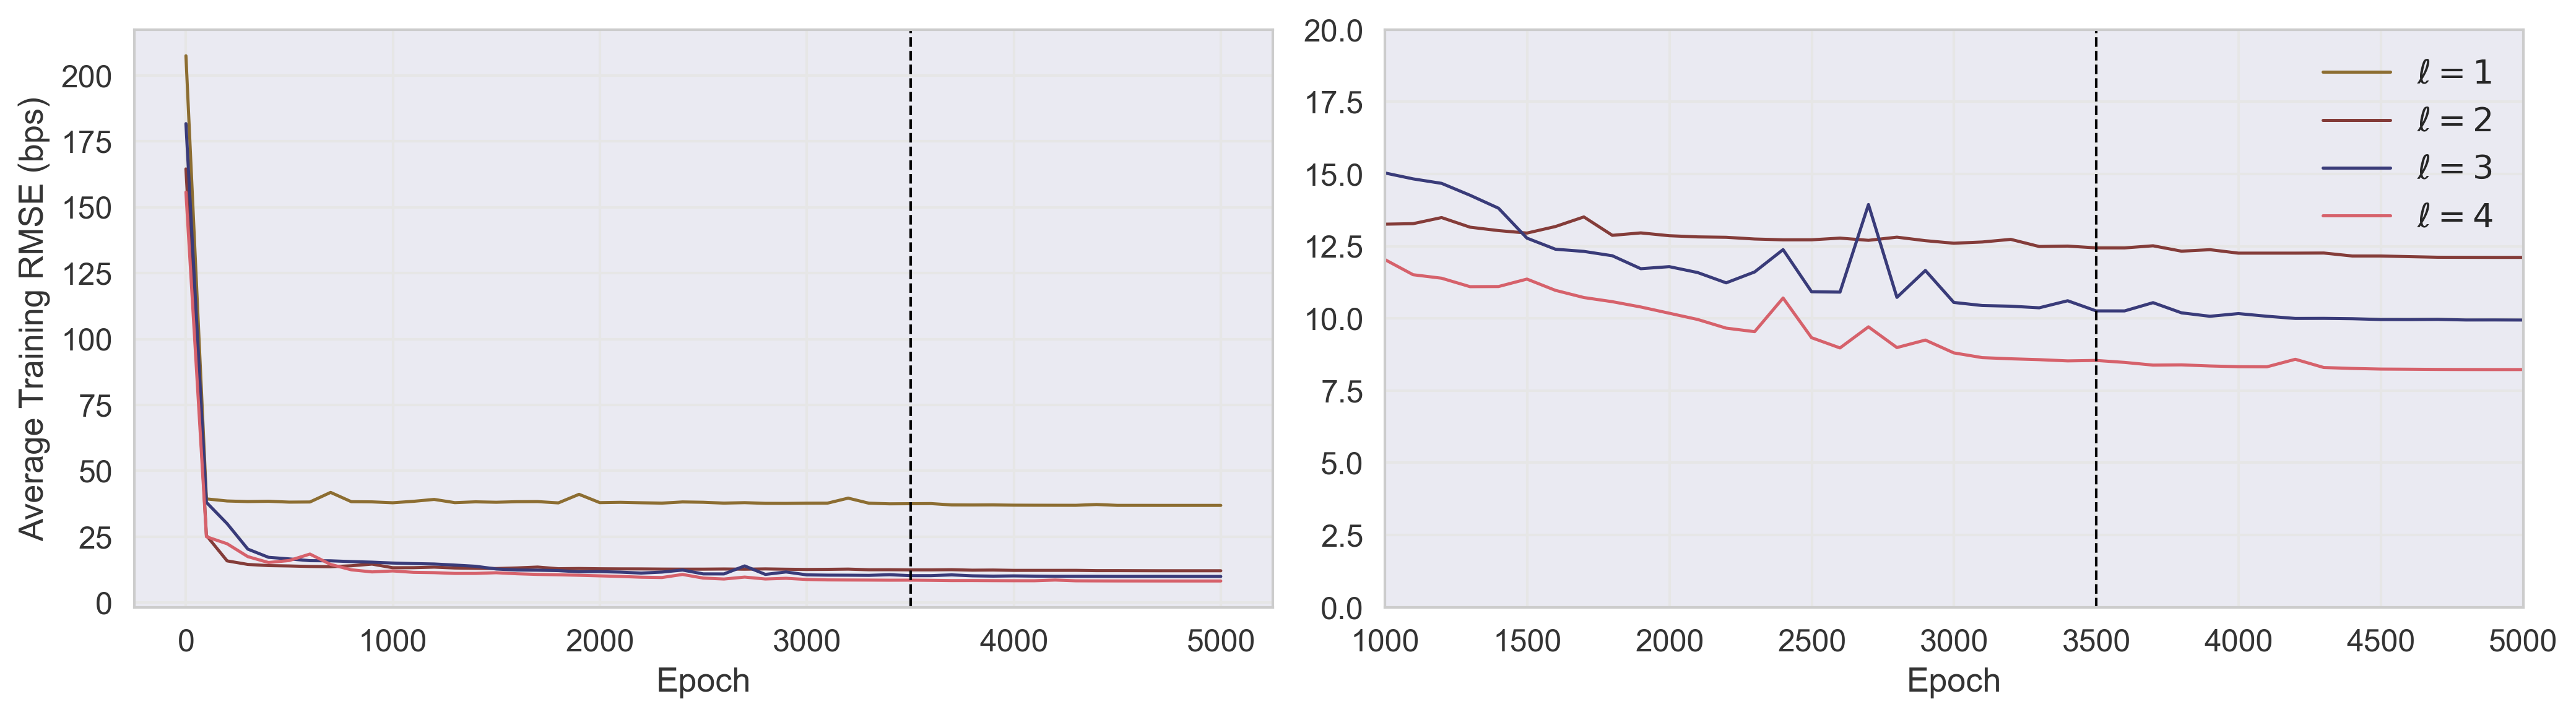
\includegraphics[width=1.03\textwidth]{Figures/thesis_results/AutoencoderPerformance/Q1e_training_loss_curves.png}
    \caption{Average in-sample training RMSE (bps) throughout 5\,000 epochs, where each curve corresponds to a separately trained model with $\ell \in \{1, 2, 3, 4\}$ latent factors, averaged across all currencies. The right panel zooms in on the region where the training loss stabilises, with the dashed vertical line marking epoch 3\,500 as the point beyond which only marginal improvements are observed.}
    \label{fig:training_loss}
\end{figure}
Table \ref{tab:q1a_is_rmse} confirms this, with $\ell=1$ yielding an average RMSE of 36.9 bps compared with 12.1 bps for $\ell=2$, indicating that a single latent factor is insufficient to capture the full shape of the swap rate curve. Given the relatively poor reconstruction accuracy of $\ell=1$, the remainder of the evaluation focuses on $\ell\in\{2,3,4\}$.

\begin{table}[h]
\centering
{\footnotesize
\pgfplotstableread[col sep=comma]{Figures/thesis_results/AutoencoderPerformance/Q1a_IS_rmse_all_dims.csv}\datqonea
\resizebox{\textwidth}{!}{%
\pgfplotstabletypeset[
  columns={index, AUD, CAD, DKK, EUR, JPY, NOK, SEK, GBP, USD, Average, Time (min)},
  columns/index/.style={column name={Model}, string type, column type=c},
  columns/AUD/.style={column type=r, fixed, precision=1, fixed zerofill},
  columns/CAD/.style={column type=r, fixed, precision=1, fixed zerofill},
  columns/DKK/.style={column type=r, fixed, precision=1, fixed zerofill},
  columns/EUR/.style={column type=r, fixed, precision=1, fixed zerofill},
  columns/JPY/.style={column type=r, fixed, precision=1, fixed zerofill},
  columns/NOK/.style={column type=r, fixed, precision=1, fixed zerofill},
  columns/SEK/.style={column type=r, fixed, precision=1, fixed zerofill},
  columns/GBP/.style={column type=r, fixed, precision=1, fixed zerofill},
  columns/USD/.style={column type=r, fixed, precision=1, fixed zerofill},
  columns/Average/.style={column name={\textbf{Avg.}}, column type=r, fixed, precision=1, fixed zerofill},
  columns/Time (min)/.style={column name={\textbf{Time}}, column type=r, fixed, precision=0, fixed zerofill},
  every head row/.style={before row=\toprule, after row=\midrule},
  every last row/.style={after row=\bottomrule},
]{\datqonea}}
}

\caption{In-sample RMSE (bps) and training time (min) for 5\,000 epochs, where each row corresponds to a separately trained model with $\ell \in \{1, 2, 3, 4\}$ latent factors. The Avg. column reports the average RMSE across all currencies.}
\label{tab:q1a_is_rmse}
\end{table}
Among the remaining models, reconstruction accuracy improves with the number of latent factors, though with diminishing gains. The average RMSE decreases from 12.1 bps for $\ell=2$ to 9.9 bps for $\ell=3$ and 8.2 bps for $\ell=4$. However, these gains come at a computational cost. Training time increases moderately from $\ell=2$ to $\ell=3$, from 58 to 63 minutes, but nearly doubles for $\ell=4$. This is largely driven by the decoder, which becomes increasingly computationaly expensive in larger latent dimensions. Specifically, the bond-pricing PDE contains the Hessian-trace term
\[
\operatorname{Tr} \left[\sigma(z_t)\sigma(z_t)^\top H_{z_t} \mathcal{G}(z_t,\tau)\right],
\]
where \(H_{z_t} \mathcal{G}\) is an \(\ell\times \ell\) Hessian, so a direct derivative calculation involves \(\mathcal{O}(\ell^2)\) second-order terms. 


The distribution of in-sample residuals, defined as the difference between the observed and reconstructed swap rates, pooled across all currencies, dates and tenors, provides further insight beyond the aggregate RMSE. As seen in Figure~\ref{fig:q1d_residual_histograms}, all three distributions are centered close to zero, indicating little systematic bias. 

\begin{figure}[h]
    \centering
    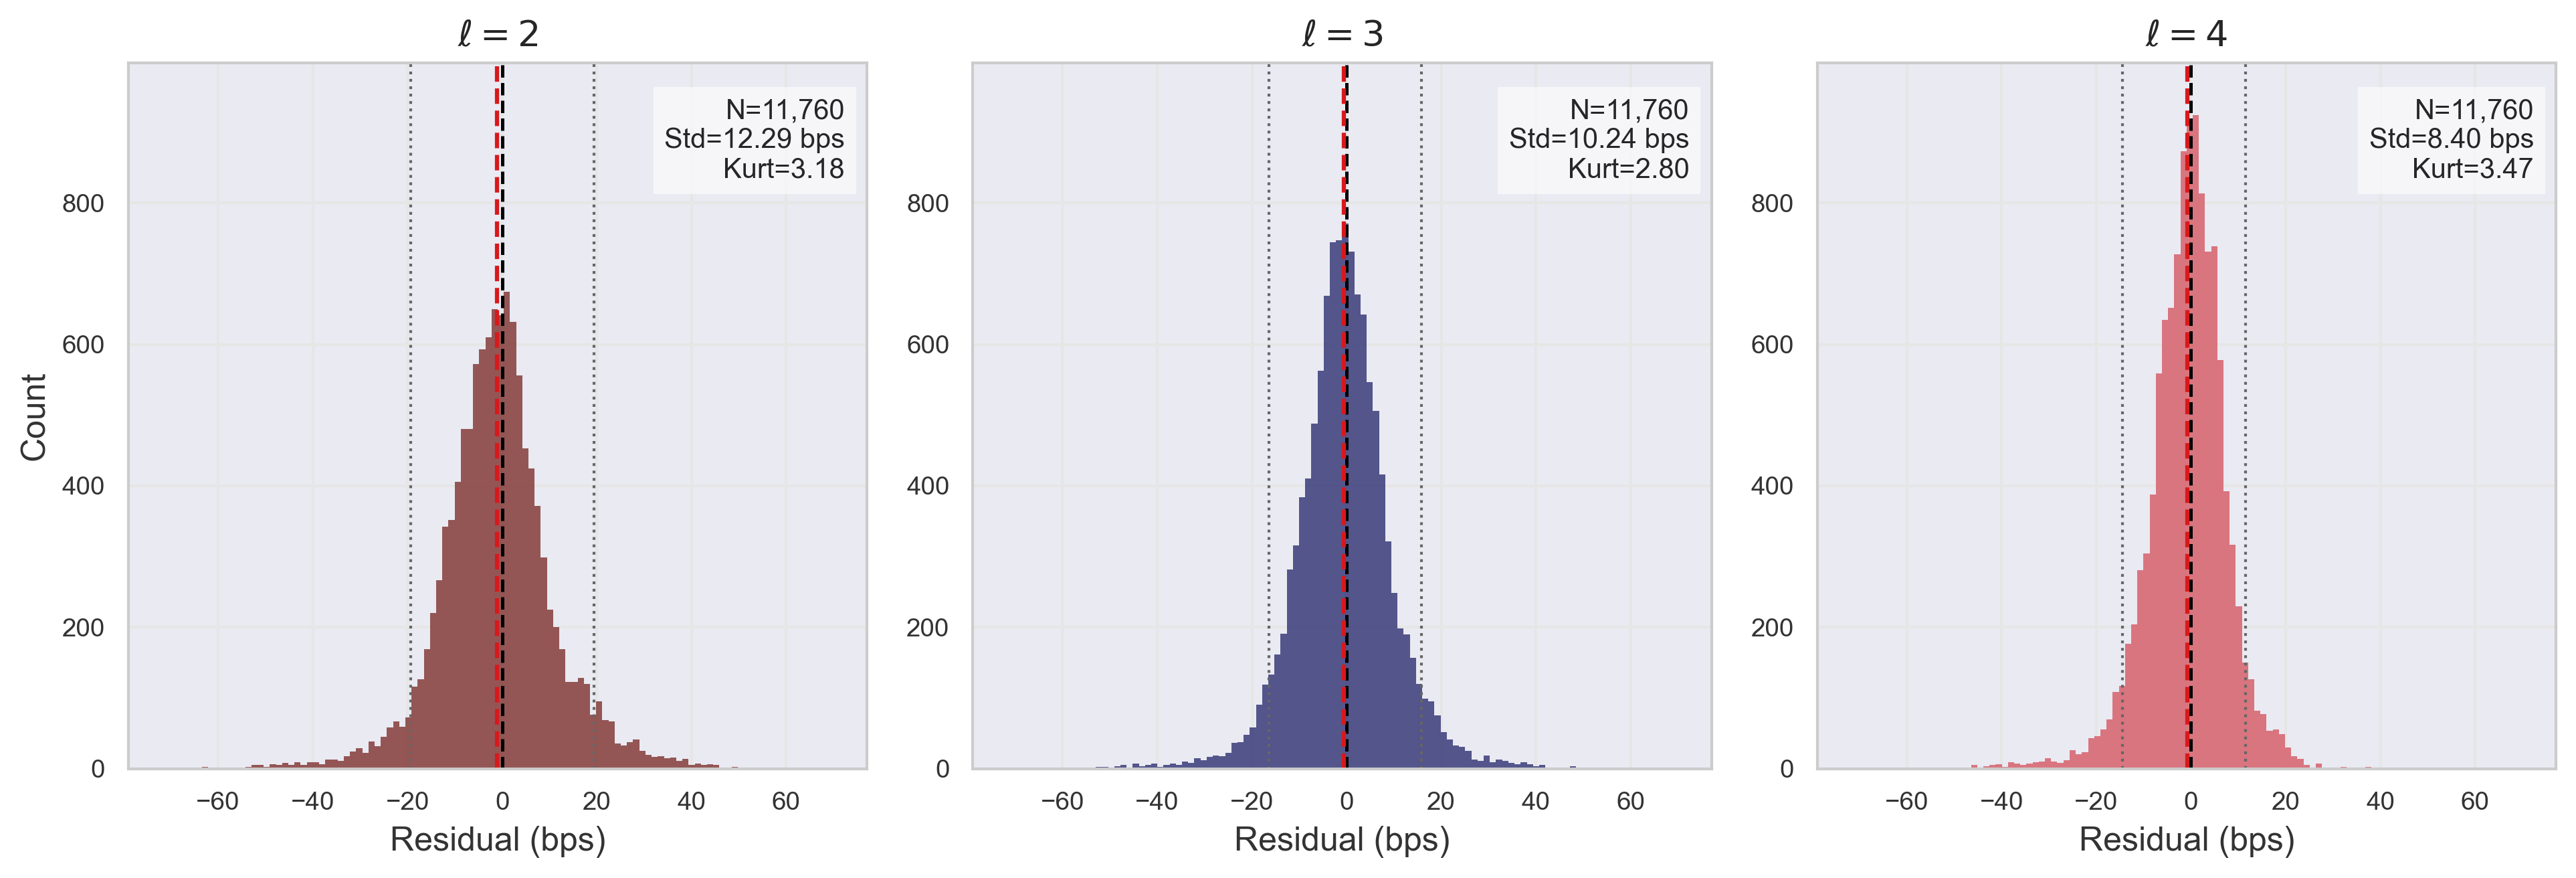
\includegraphics[width=1.0\textwidth]{Figures/thesis_results/AutoencoderPerformance/Q1d_residual_histograms_all_dims.png}
    %\caption{In-sample residual distributions for models with $\ell \in \{2, 3, 4\}$ latent factors, pooled across all currencies, dates, and maturities. The black and red dashed lines mark zero and the sample mean, respectively, while the grey dotted lines mark the 5th and 95th percentiles. Standard deviation and excess kurtosis are reported in the upper-right corner of each panel.}
    \caption{In-sample residual distributions for models with $\ell \in \{2, 3, 4\}$ latent factors, pooled across all currencies, dates, and maturities. The black and red dashed lines mark zero and the sample mean, respectively, while the grey dotted lines mark the 5th and 95th percentiles. Standard deviation and excess kurtosis are reported in the upper-right corner of each panel. All distributions are centred close to zero, indicating little systematic bias, and tighten with increasing latent dimension.}
\label{fig:q1d_residual_histograms}
\end{figure}

Higher latent dimensions yield tighter residual distributions, with the standard deviation decreasing from 12.39 bps for $\ell=2$ to 10.28 bps for $\ell=3$ and 8.40 bps for $\ell=4$ consistent with the declining RMSE reported in Table \ref{tab:q1a_is_rmse}. Nevertheless, this pooling may mask systematic errors within specific currencies, maturities, or time periods, which is addressed in what follows.


For $\ell=2$, reconstruction error is not evenly distributed over time. Around the time of the COVID-19 pandemic outbreak in March 2020, the error spikes notably for EUR and DKK, as shown in Figure~\ref{fig:Q6b}. This coincides with the sharp reversal in global swap rates observed around 2020 (Figure~\ref{fig:D2b_10y_timeseries}, Chapter~\ref{chap:datadescription}), suggesting that the model may struggle to reconstruct curves during periods of regime change, particularly given that it was trained on a predominantly globally declining rate environment.
\begin{figure}[H]
    \centering
    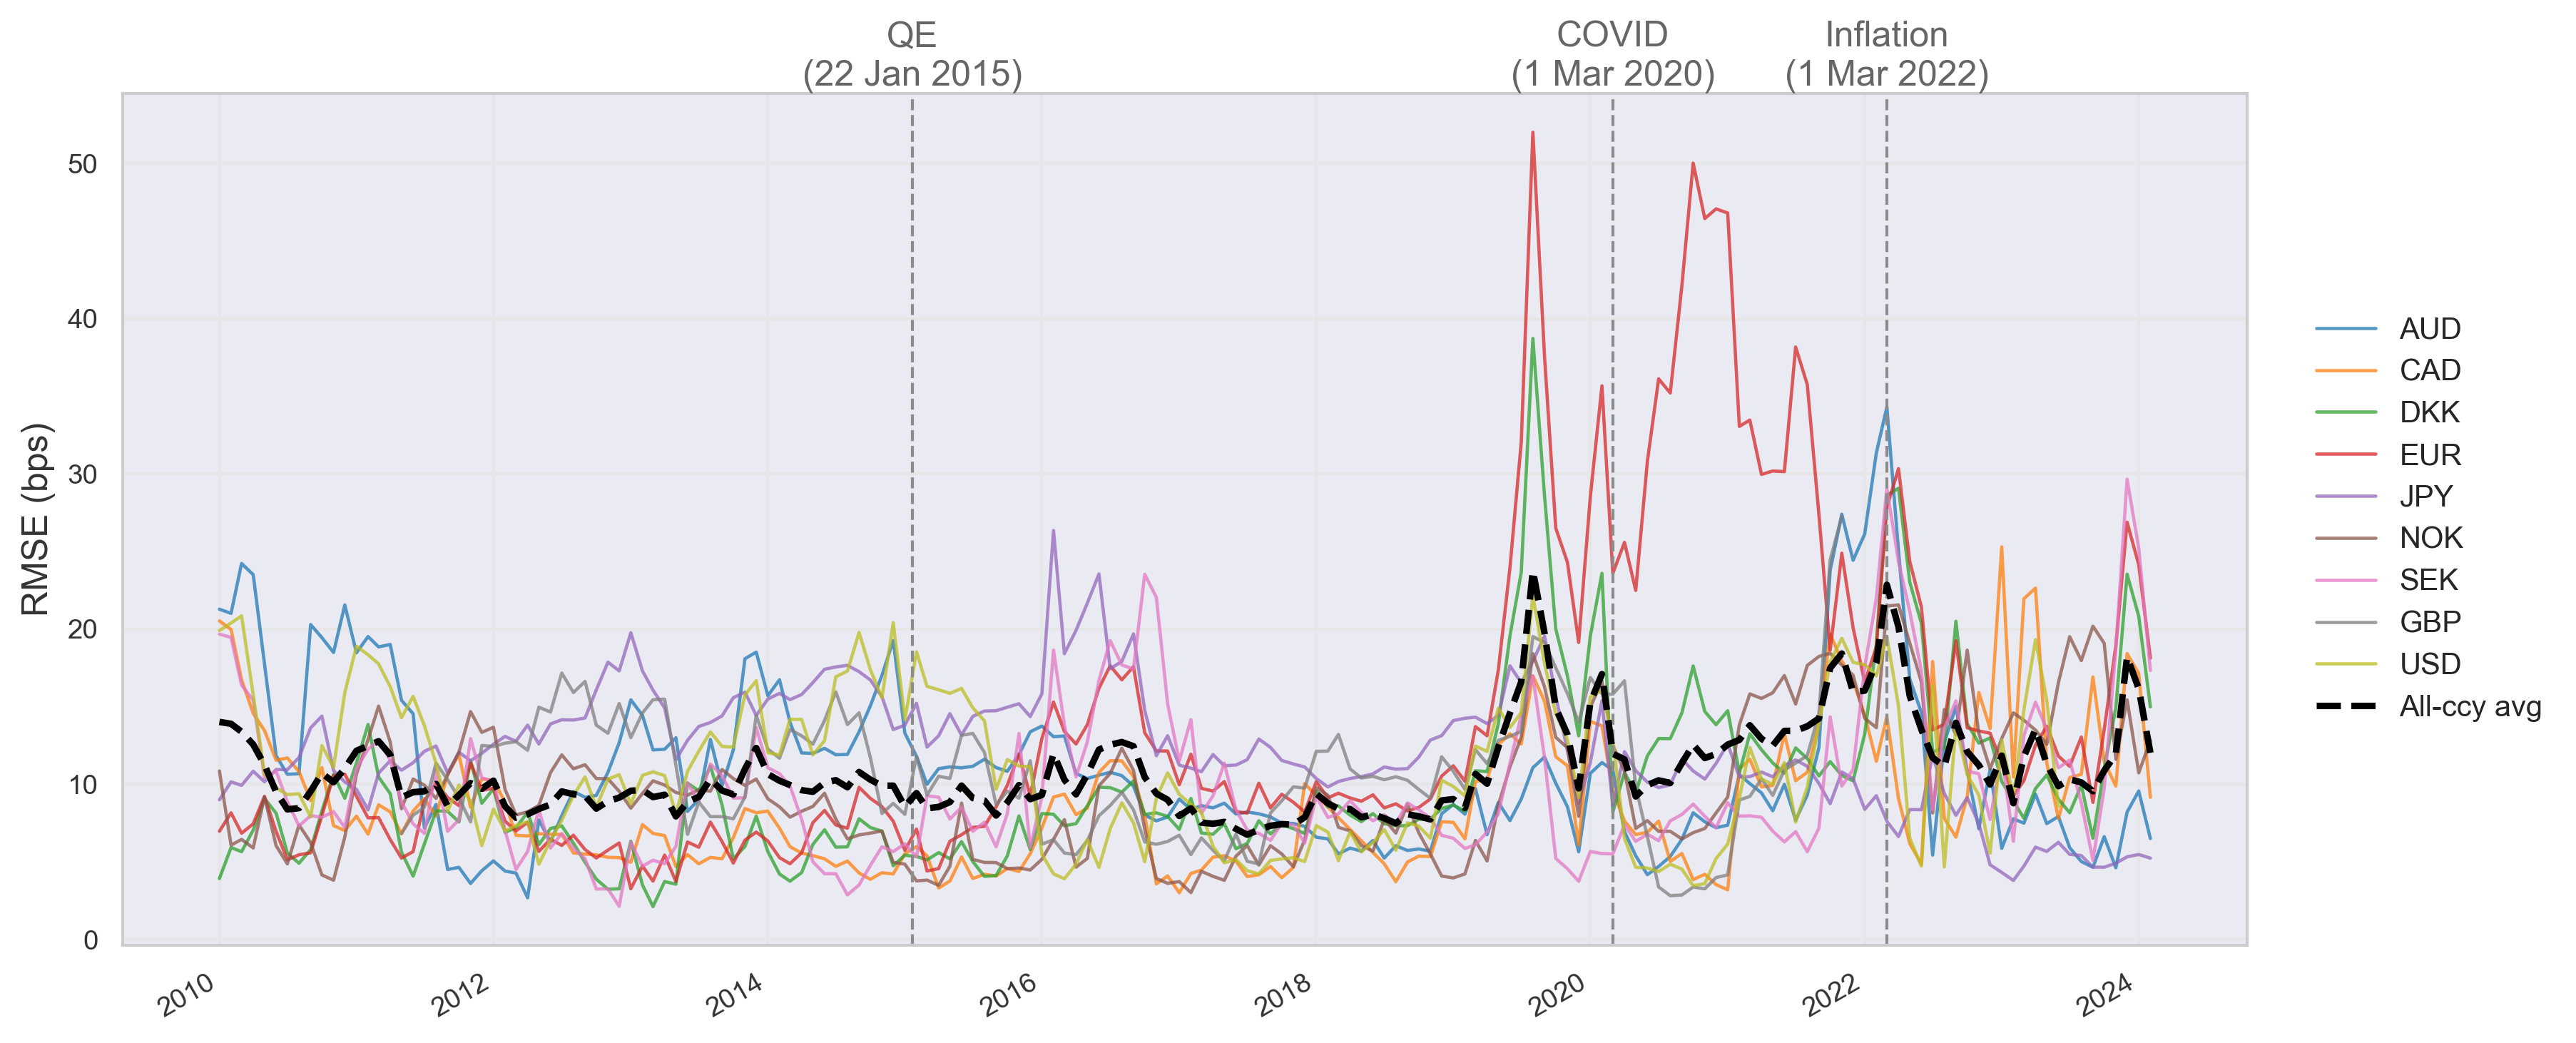
\includegraphics[width=1.00\textwidth]{Figures/thesis_results/AutoencoderPerformance/Q6b_rmse_over_time.png}
    %\caption{In-sample RMSE (bps) over the full sample period for the model with $\ell = 2$ latent factors, shown per currency alongside the cross-currency average (black dashed line). Vertical dashed lines indicate the onset of macroeconomic regimes.}
    \caption{In-sample RMSE (bps) over the full sample period for the model with $\ell = 2$ latent factors, shown per currency alongside the cross-currency average (black dashed line). Vertical dashed lines indicate the onset of macroeconomic regimes. \textcolor{red}{Reconstruction errors remain low for most of the sample but rise around the COVID outbreak in 2020, suggesting that the model struggles when the rate environment differs from the period on which it was trained.}}
    \label{fig:Q6b}
\end{figure}
Beyond the time dimension, reconstruction error also varies systematically across maturities. Figure~\ref{fig:Q6a} shows that the short and long ends of the swap rate curve are consistently more difficult to reconstruct across all models, while mid-range maturities exhibit lower errors. This may reflect the fact that the encoder--decoder has less structural information to draw on at the boundaries of the maturity spectrum, where the curve shape is more sensitive to short-term monetary policy expectations at the short end and to long-run term premium dynamics at the long end. The effect is most pronounced at the short end, with EUR and JPY exhibiting the largest errors at these extremes, consistent with their higher RMSE in Table~\ref{tab:q1a_is_rmse}.
% Kunne det ikke også have noget at gøre med at modellen fanger level bedre, og så derfor passe bedre med midtpunktet?
\begin{figure}[h]
    \centering
    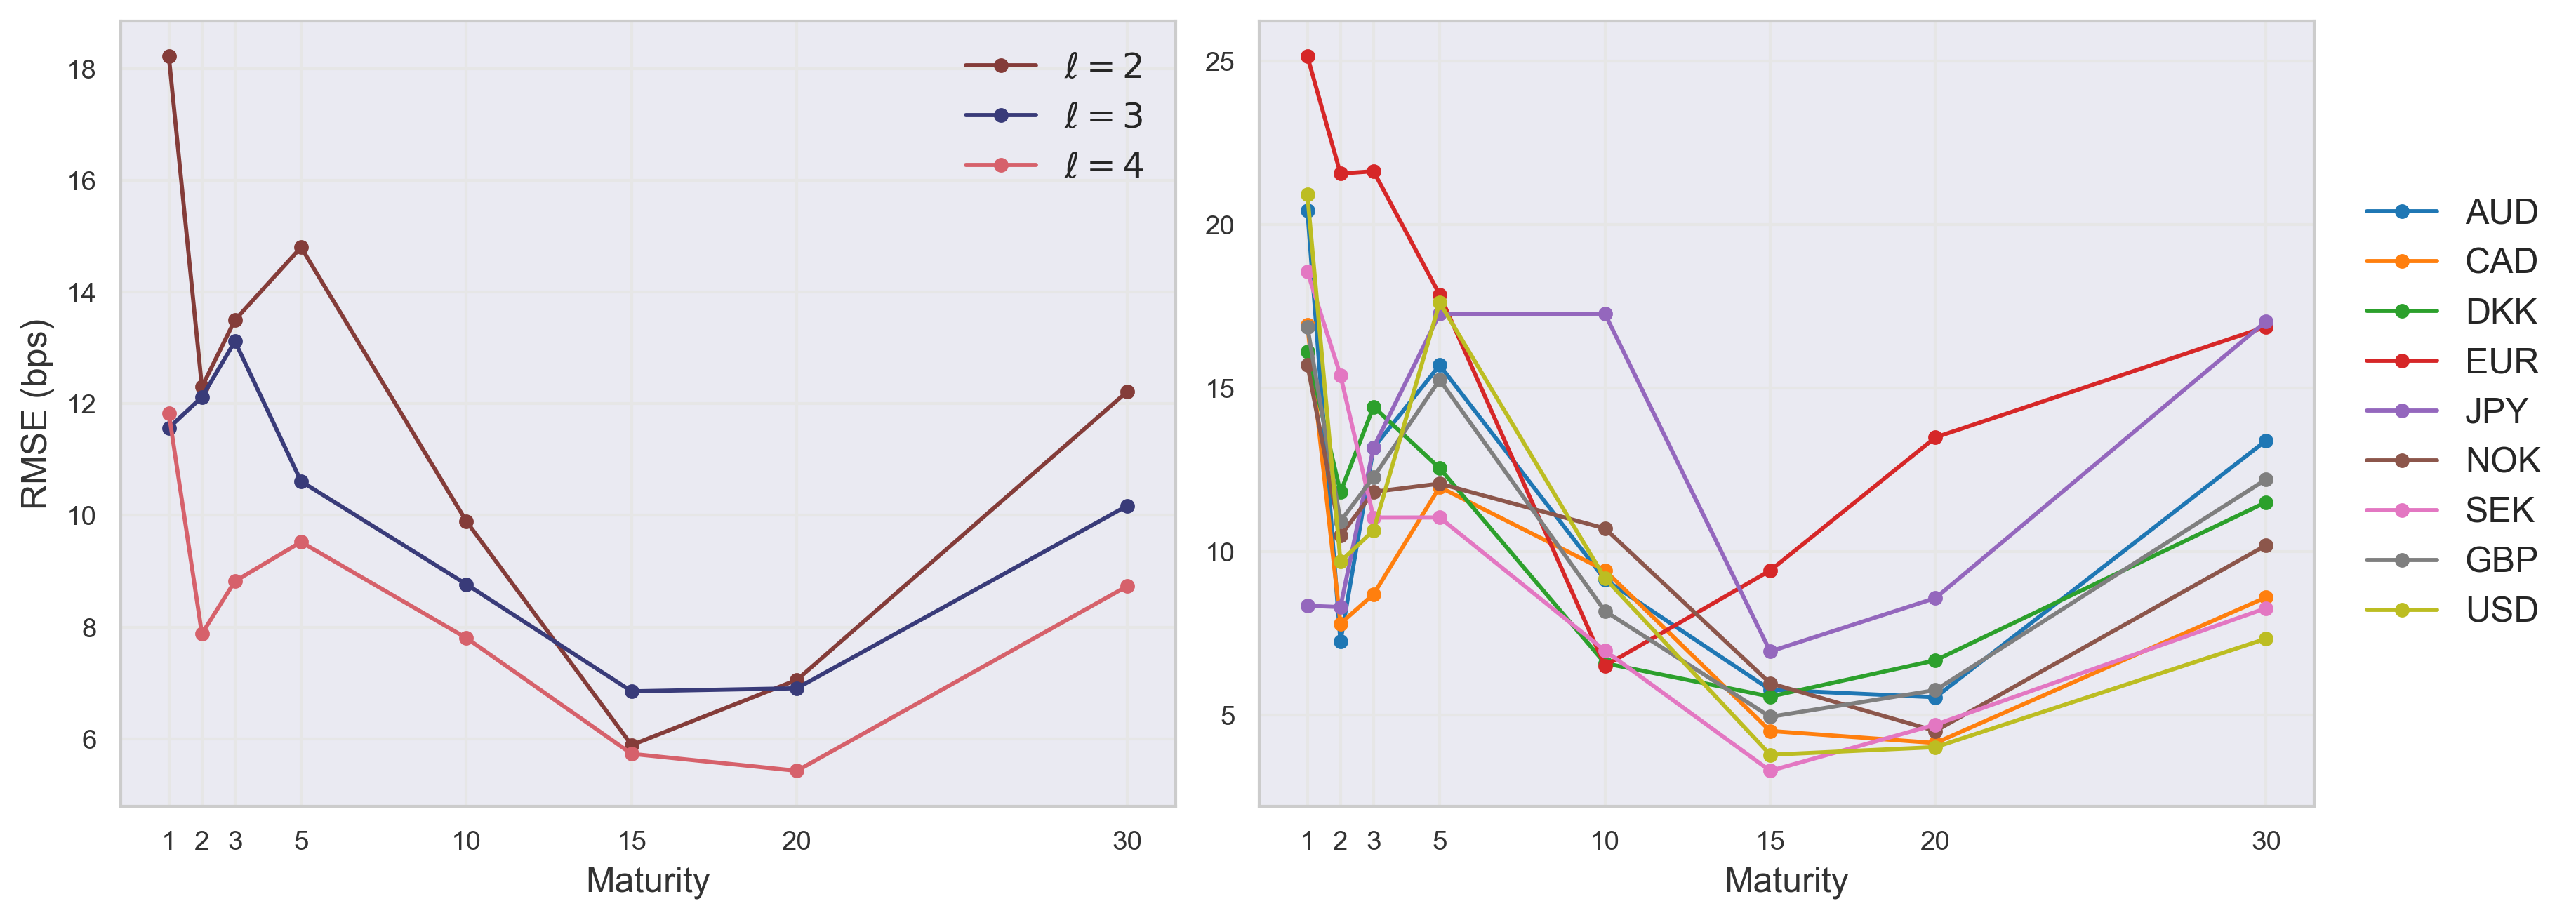
\includegraphics[width=1.0\textwidth]{Figures/thesis_results/AutoencoderPerformance/Q6a_rmse_by_tenor.png}
    %\caption{In-sample RMSE (bps) by maturity, averaged across all currencies and dates, for models with $\ell \in \{2, 3, 4\}$ latent factors (left). The right panel shows the same for $\ell = 2$ broken down per currency, averaged across dates.}
    \caption{In-sample RMSE (bps) by maturity, averaged across all currencies and dates, for models with $\ell \in \{2, 3, 4\}$ latent factors (left). The right panel shows the same for \(\ell =2\) broken down per currency, averaged across dates. Reconstruction error is consistently highest at the short and long ends of the maturity spectrum across all models, while mid-range maturities are reconstructed most accurately.}
    \label{fig:Q6a}
\end{figure}

Moving beyond aggregate error measures, Figure~\ref{fig:Q1d} visualises the fit of the reconstructed swap rate curves across different market regimes. Two representative dates are shown. One during a \textit{calmer} market environment in August 2014 and the other during the COVID-19 pandemic outbreak in March 2020.

\begin{figure}[h]
    \centering
    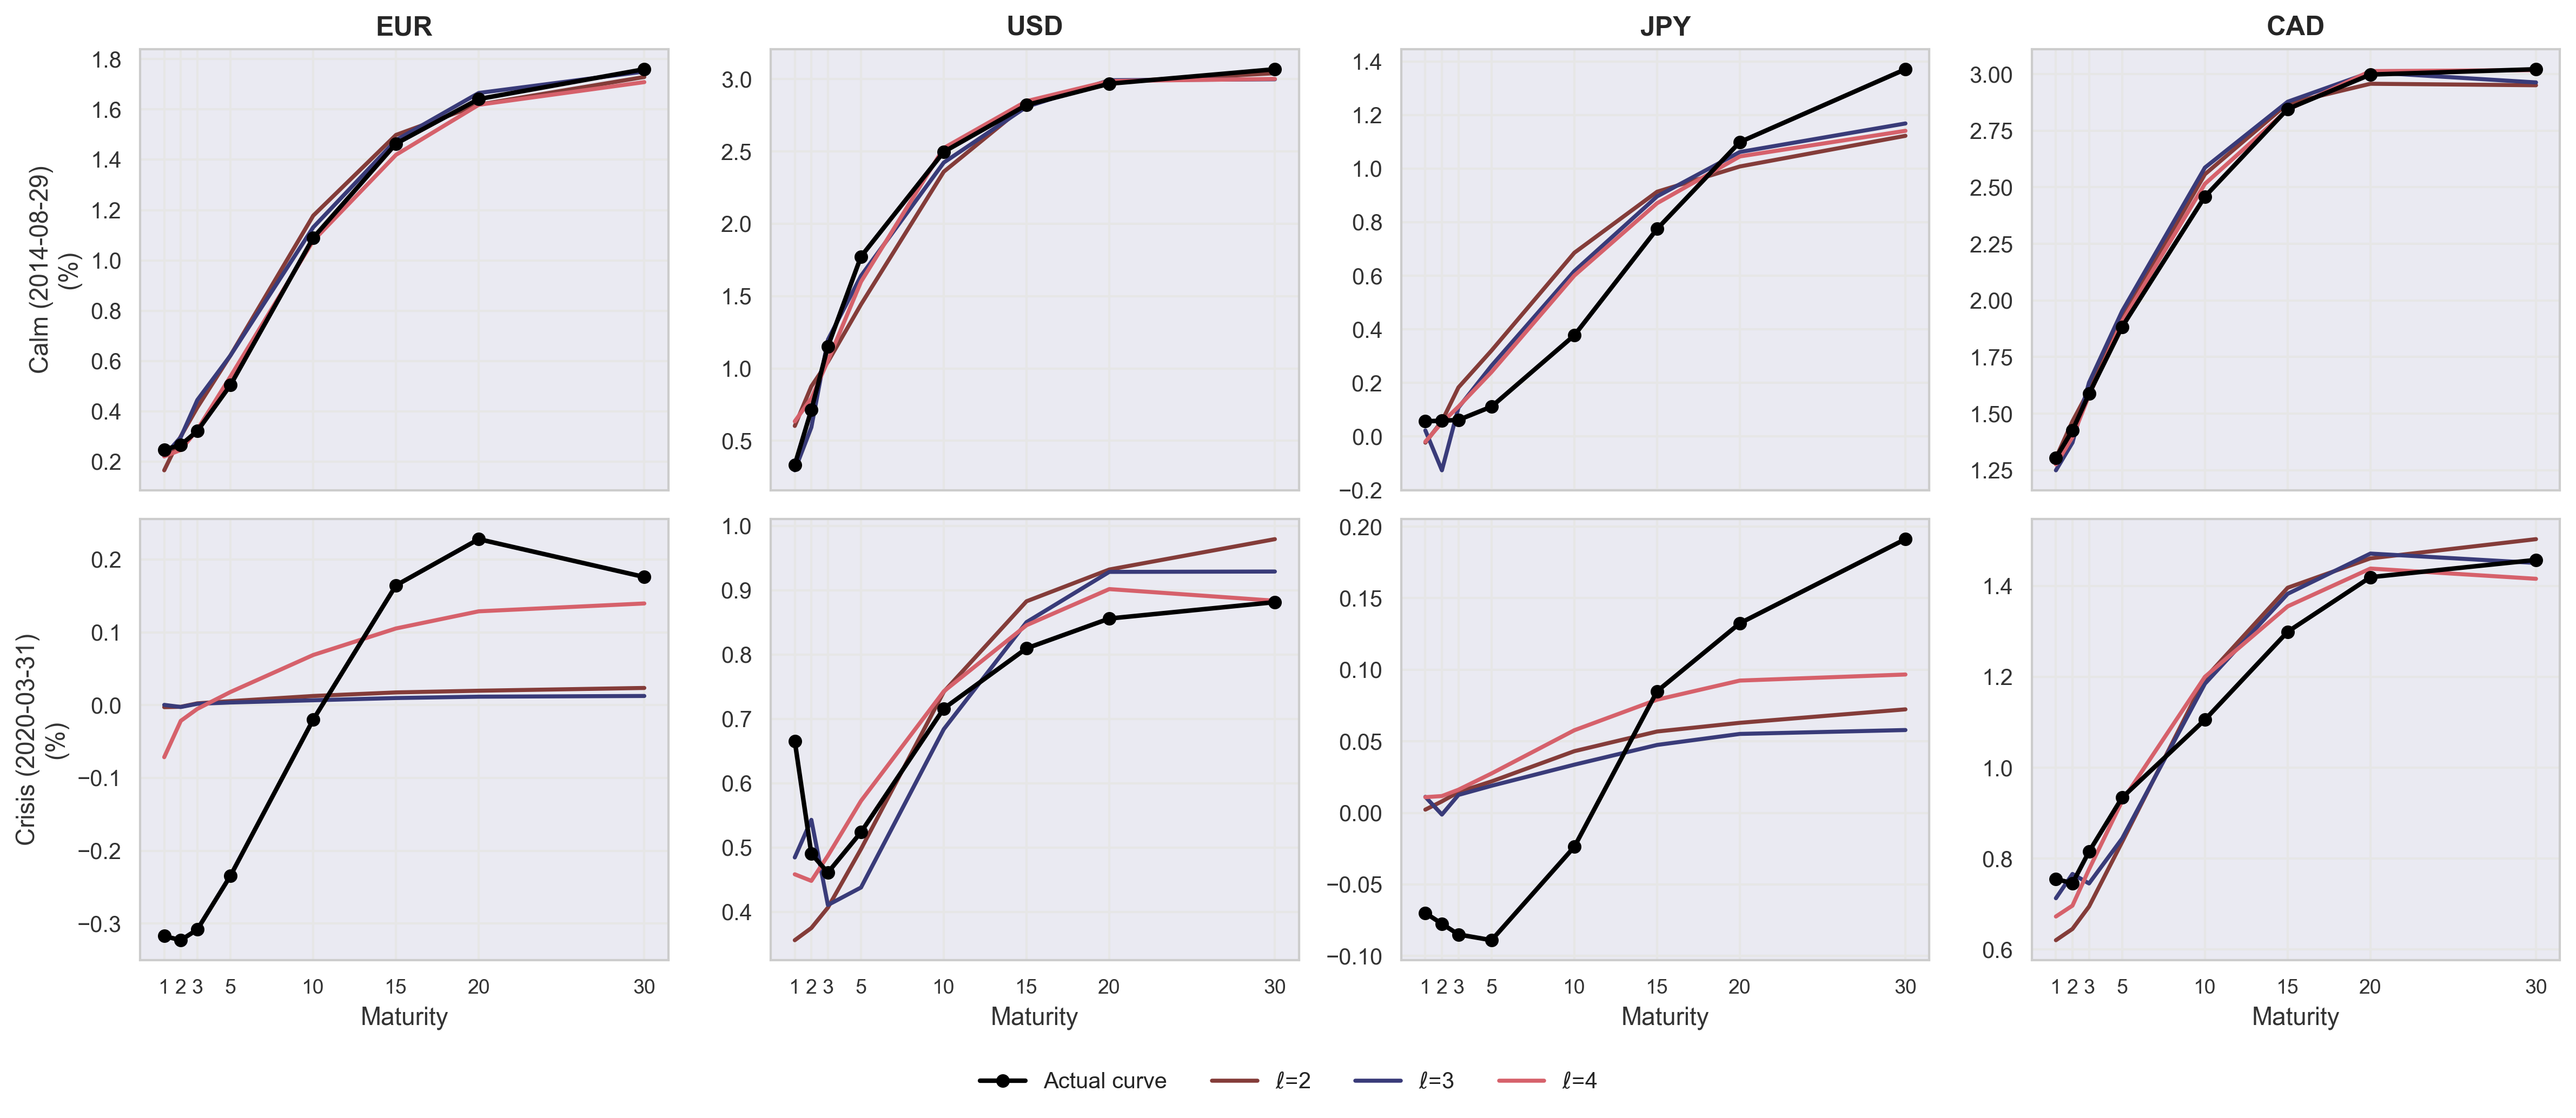
\includegraphics[width=\textwidth]{Figures/thesis_results/AutoencoderPerformance/Q1d_fitted_vs_actual_all_dims.png}
    %\caption{Comparison of actual swap curves against reconstructed curves for models with $\ell \in \{2, 3, 4\}$ latent factors, across a calm date (2014-08-29) and a crisis date during the COVID regime (2020-03-31) for EUR, USD, JPY, and CAD.}
    \caption{Comparison of actual swap curves against reconstructed curves for models with $\ell \in \{2, 3, 4\}$ latent factors, across a calm date (2014-08-29) and a crisis date during the COVID regime (2020-03-31) for EUR, USD, JPY, and CAD. Reconstruction is accurate during the calm period, but during the crisis, EUR and JPY are poorly fitted, with the model capturing the level while missing slope and curvature. This pattern is consistent across all latent dimensions, \textcolor{red}{ ( suggesting a fundamental limitation of the model rather than a consequence of dimensionality.) / ( pointing to a structural limitation of the encoder.)}}
    \label{fig:Q1d}
\end{figure}

During the calmer period, the observed curves are generally reconstructed well across all models, although JPY exhibits mismatch at both the short and long ends. Reconstruction becomes more challenging for curves from the COVID-19 outbreak period, particularly for EUR and JPY, where all three models struggle similarly. For these currencies, observed swap rates reach negative levels at the short end and slope upward to positive but still very low levels at the long end. The fitted curves across all models, however, remain flat and close to zero, capturing the level, but failing to reproduce the slope and curvature. Since this limitation persists regardless of the number of latent factors, it points to a more fundamental constraint of the encoder-decoder framework, rather than a consequence of the choice of latent dimension. This inability to capture slope and curvature is further examined in Chapter \ref{chap:model_comparison}.

It is of interest to examine whether the models not only struggle with negative rate curves, but also inverted curves. To investigate this, the per-curve RMSE is plotted over time in Figure~\ref{fig:q6e_scatter_regime}, coloured by curve type, where each curve is classified as either normal, inverted or negative (see Table \ref{tab:curve_type_counts}). Normal curves are reconstructed most accurately, while inverted and negative-rate curves exhibit notably higher errors, suggesting that the model struggles to reconstruct curve shapes that are underrepresented in the training data.


\begin{figure}[H]
    \centering
    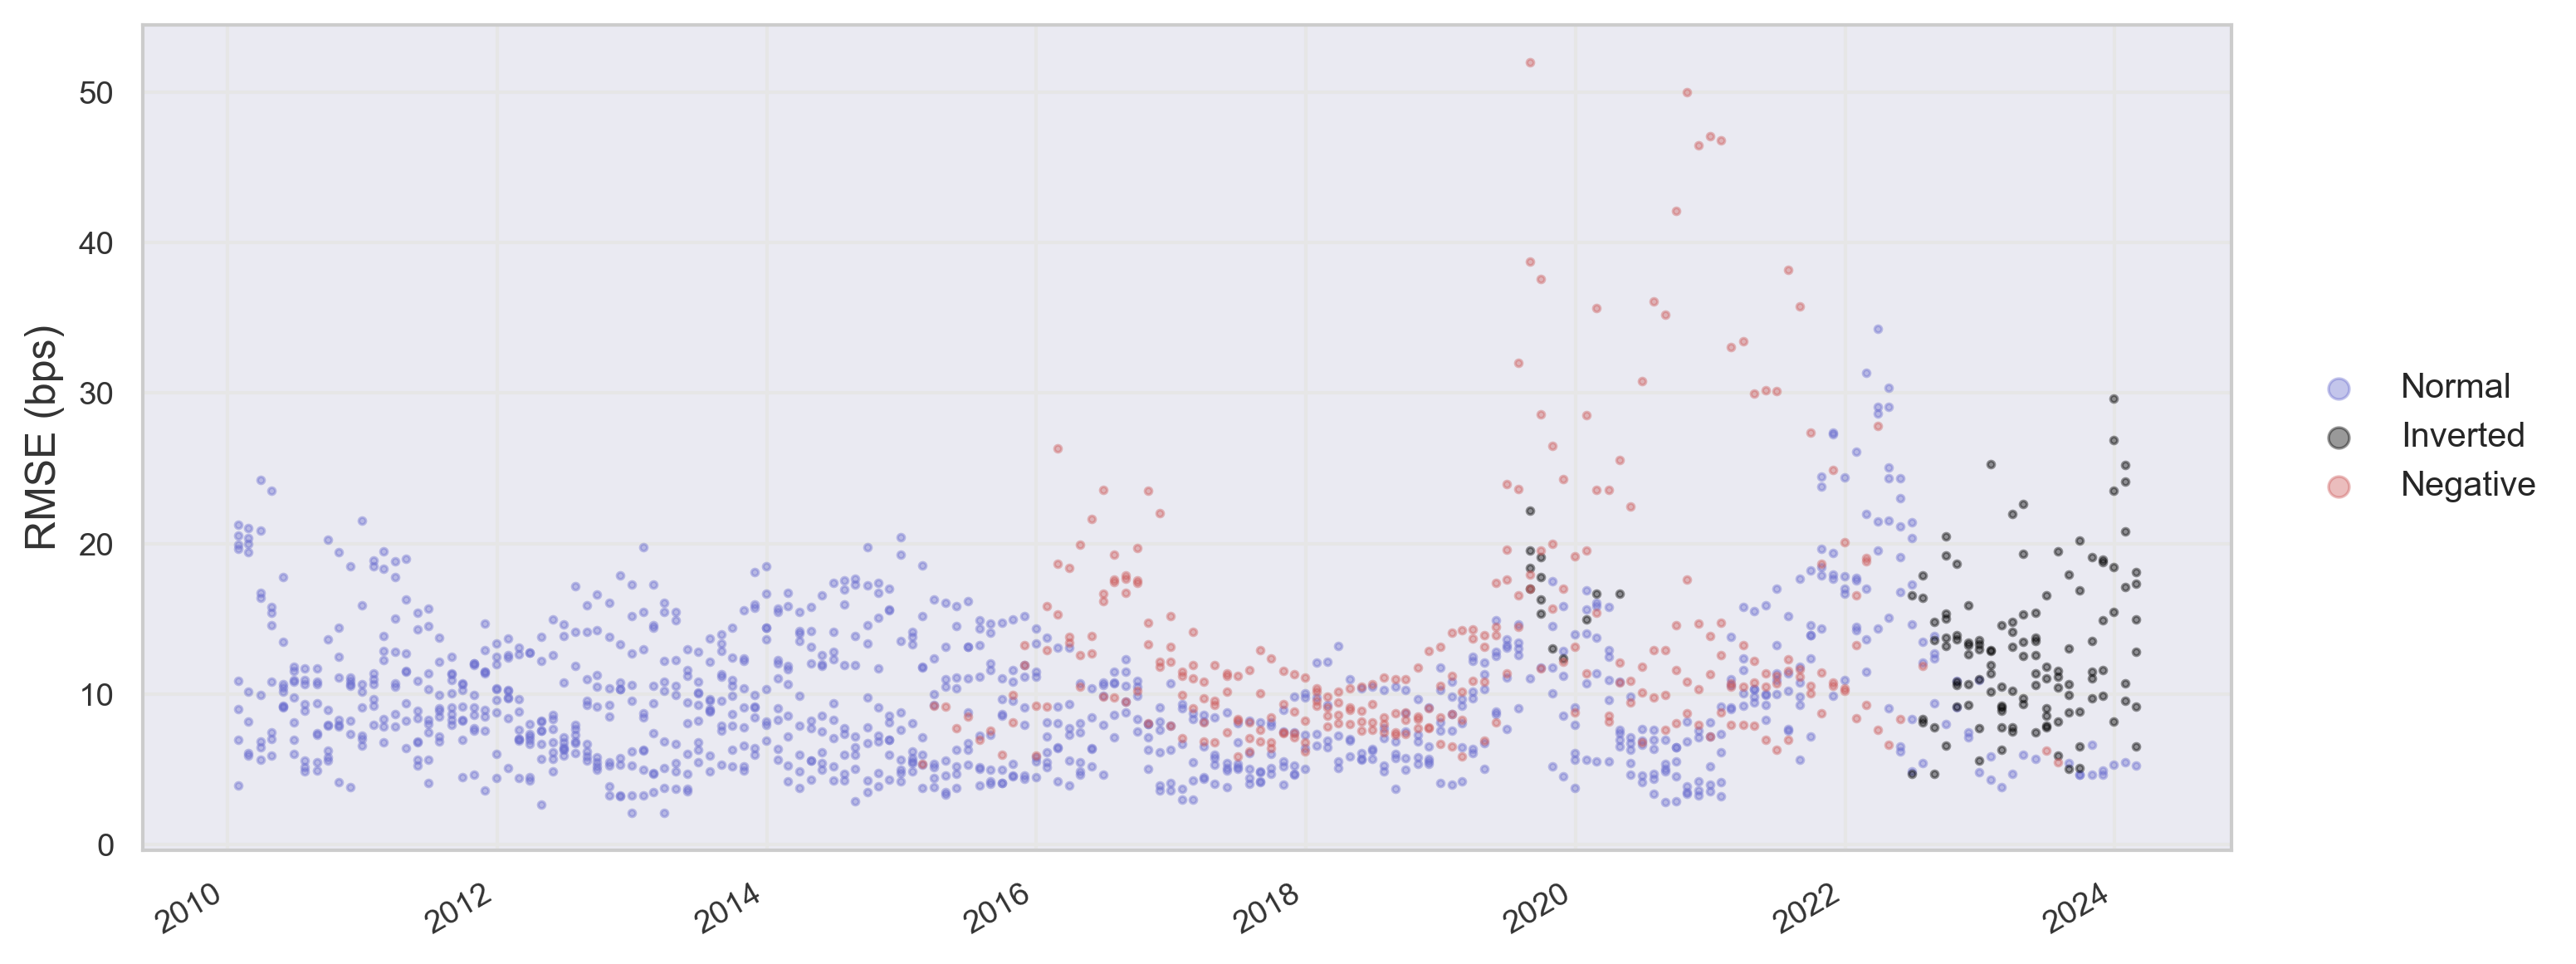
\includegraphics[width=1.0\textwidth]{Figures/thesis_results/AutoencoderPerformance/Q6e_scatter_regime.png}
    %\caption{Per-observation in-sample RMSE (bps) over time for the model with $\ell = 2$ latent factors, coloured by curve type (see Table~\ref{tab:curve_type_counts}). Each point reports the reconstruction error for a single curve observation, pooled across all currencies.}
    \caption{Per-observation in-sample RMSE (bps) over time for the model with $\ell = 2$ latent factors, coloured by curve type. Each point reports the reconstruction error for a single curve observation, pooled across all currencies. Normal curves are reconstructed most accurately, while inverted and negative-rate curves show consistently higher errors, reflecting their underrepresentation in training.}
\label{fig:q6e_scatter_regime}
\end{figure}

%Table~\ref{tab:q6e_combined} quantifies this. Normal, non-negative curves account for the majority of observations and are reconstructed with an average RMSE of 7.62 bps, compared to 12.53 bps for inverted curves and 12.60 bps for negative-rate curves, representing roughly a 65\% increase in reconstruction error across both regimes.

%\begin{table}[H]
%\centering
%{\small
%\pgfplotstableread[col sep=comma, trim cells=true]{Figures/thesis_results/AutoencoderPerformance/Q6e_rmse_combined_display.csv}\datqsixe
%\resizebox{\textwidth}{!}{%
%\pgfplotstabletypeset[
%  columns={Curve Variant, Metric, AUD, CAD, DKK, EUR, JPY, NOK, SEK, GBP, USD, All},
%  columns/Curve Variant/.style={column name={Curve Variant}, string type, column type=l},
%  columns/Metric/.style={column name={Metric}, string type, column type=l},
%  columns/AUD/.style={string type, column type=r},
%  columns/CAD/.style={string type, column type=r},
%  columns/DKK/.style={string type, column type=r},
%  columns/EUR/.style={string type, column type=r},
%  columns/JPY/.style={string type, column type=r},
%  columns/NOK/.style={string type, column type=r},
%  columns/SEK/.style={string type, column type=r},
%  columns/GBP/.style={string type, column type=r},
%  columns/USD/.style={string type, column type=r},
%  columns/All/.style={column name={\textbf{All}}, string type, column type=r},
%  every head row/.style={before row=\toprule, after row=\midrule},
%  every row no 1/.style={after row=\midrule},
%  every row no 3/.style={after row=\midrule},
%  every last row/.style={after row=\bottomrule},
%]{\datqsixe}}
%}
%\caption{In-sample RMSE (bps) by interest rate regime for the baseline autoencoder with $\ell=3$ latent factors. Observations are classified as \textit{inverted} when the short end exceeds the long end, and as \textit{negative} when any tenor is below zero. $N$ denotes the number of curve observations in each regime. The \textit{Inverted, Negative} regime contains no observations in the estimation sample.}
%\label{tab:q6e_combined}
%\end{table}



%The in-sample reconstruction results show that the autoencoder captures swap rate curves with o accuracy once at least two latent factors are used. Increasing the latent dimension improves reconstruction accuracy, though with diminishing gains. The remaining errors are concentrated at the short and long ends of the curve, during periods of abrupt market movements, and for structurally atypical curve shapes such as inverted and negative-rate curves. The latter is particularly evident for EUR and JPY during the COVID-19 shock. 

In addition to reconstruction accuracy, we examine whether the model-implied short rate $\tilde r(z_t)$ is economically reasonable. 

\begin{figure}[H]
    \centering
    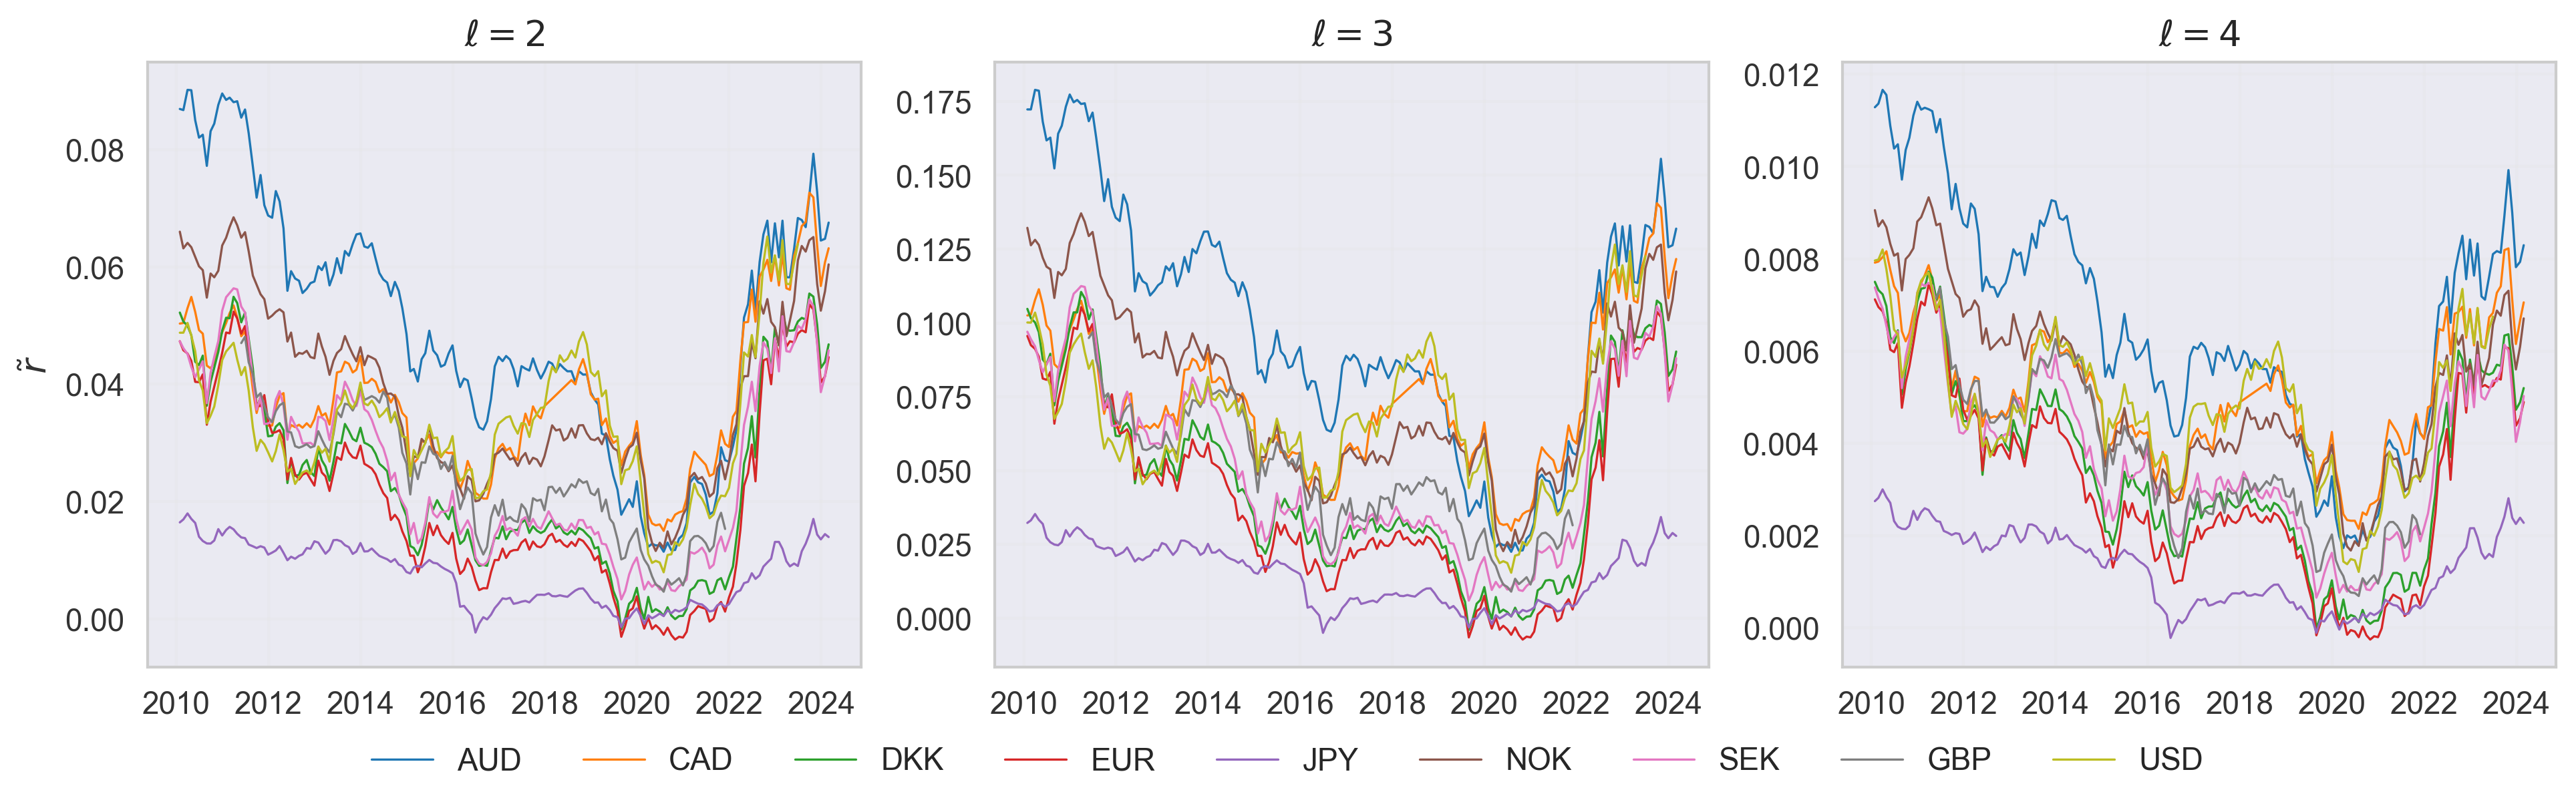
\includegraphics[width=\textwidth]{Figures/thesis_results/AutoencoderPerformance/r_tilde_all_dims.png}
    %\caption{Model-implied short rate $\tilde{r}(z_t)$ over the full in-sample period for models with $\ell \in \{2, 3, 4\}$ latent factors. Note that the vertical axis differs across panels.}
    \caption{Model-implied short rate $\tilde{r}(z_t)$ over the full in-sample period for models with $\ell \in \{2, 3, 4\}$ latent factors. Note that the vertical axis differs across panels. All models share the same broad trajectory, but the level and scale differ across latent dimensions, as the short rate is learned implicitly through the reconstruction loss rather than calibrated to an observed market rate.}
    \label{fig:r_tilde_all_dims}
\end{figure}

As shown in Figure \ref{fig:r_tilde_all_dims}, the implied short rates share a consistent trajectory across all models, declining toward the low-rate environment of 2019--2020 and rising sharply from 2022 onwards, yet the level and scale differ substantially. The $\ell=3$ model produces considerably higher short-rate levels, while the $\ell=4$ model produces a short rate in a much narrower range.

Since the short rate is learned implicitly through the swap-rate reconstruction loss rather than calibrated to an observed overnight or policy rate, the model has no explicit incentive to produce economically meaningful short-rate levels. This is consistent with the finding in Figure~\ref{fig:Q6a} that the short end of the curve is systematically the hardest to reconstruct, suggesting that the model has limited structural information about short-maturity dynamics and thus little basis for anchoring the short rate to economically meaningful levels. The implied short rate should therefore be interpreted as a model-implied quantity, rather than as a direct estimate of the market short rate.





%Across all three models, the implied short rates move in the same overall direction as the observed swap rates over the sample period. They decline toward the low-rate period around 2019--2020 and rise sharply from 2022 onwards. The level and scale of the implied short rate, however, vary substantially across latent dimensions. In particular, the $\ell=3$ model produces much higher short-rate levels, while the $\ell=4$ model compresses the short rate into a much narrower range.

%Although the short rate is explicitly modelled as a function of the latent state, it is learned through the swap-rate reconstruction loss rather than by direct calibration to an observed overnight or policy rate. This may partly explain why the implied short-rate levels differ across latent dimensions, even when the reconstructed swap curves are similar. The implied short rate should therefore be interpreted with some caution as a model-implied component of the arbitrage-free decoder, rather than as a separately calibrated estimate of the market short rate.




\subsection{No-Arbitrage PDE Residual Diagnostic}

We next verify that the models satisfies the no-arbitrage condition by computing the residual of the bond-pricing PDE in \eqref{eq:bond_pricing_pde}. Since the decoder constructs zero-coupon bond prices by solving the ODE system derived from this PDE, the residual should be close to zero up to numerical approximation error.

\begin{figure}[H]
    \centering
    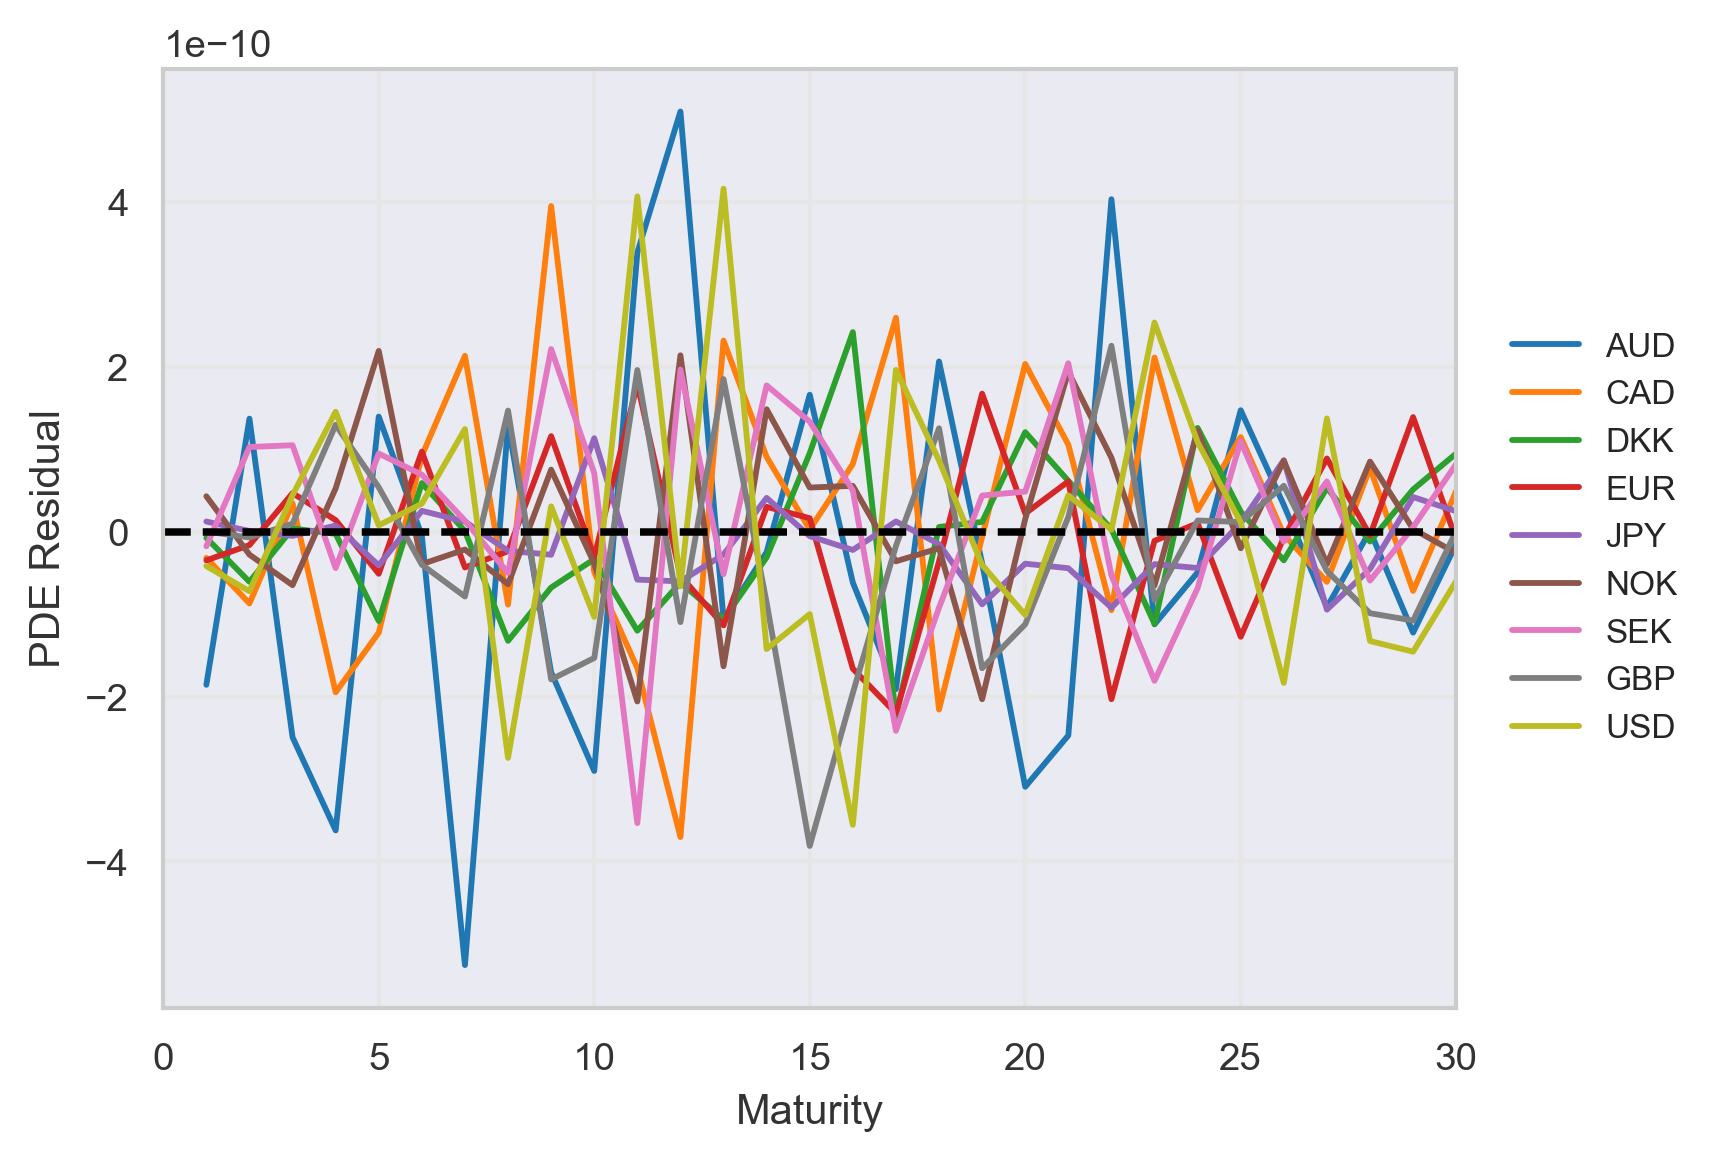
\includegraphics[width=0.7\textwidth]{Figures/thesis_results/AutoencoderPerformance/Q7_sharpe_ratio_IS_dim2.png}
    \caption{Bond-pricing PDE residual $R(\tau)$ (Equation~\ref{eq:pde_residual}) as a function of maturity for the model with $\ell = 2$ latent factors, averaged across in-sample observations per currency. Residuals are of order $10^{-10}$, indicating that the no-arbitrage pricing condition is satisfied to numerical precision.}
\label{fig:Q7_pde_residual}
    \label{fig:Q7_pde_residual}
\end{figure}

%The figure reports the diagnostic for $\ell=3$ as the representative specification. As the same ODE-based construction is used across latent dimensions, the same diagnostic can be applied to $\ell=2$ and $\ell=4$ to verify numerical satisfaction of the no-arbitrage PDE across specifications.

The diagnostic is reported for the $\ell=2$ model in Figure~\ref{fig:Q7_pde_residual}, averaged by currency over all in-sample dates. Two features indicate that the no-arbitrage condition is satisfied numerically. First, the residuals are on the order of $10^{-10}$, so deviations from zero are negligible in magnitude. Second, the values fluctuate randomly around zero across all maturities and currencies, consistent with numerical noise rather than a systematic arbitrage violation. The same result holds for the $\ell=3$ and $\ell=4$ models, and the no-arbitrage restriction is therefore satisfied numerically across all models.








% ─────────────────────────────────────────────────────────────
\section{Out-of-Sample Evaluation}
% ─────────────────────────────────────────────────────────────

Accurate in-sample reconstruction is necessary but not sufficient for generalisation to unseen swap rate curves. To assess whether the arbitrage-free encoder--decoder generalises beyond a training sample, we evaluate its out-of-sample reconstruction performance using a rolling window scheme. Based on the convergence analysis in Figure~\ref{fig:training_loss}, each model is trained over 3\,500 epochs.\footnote{The rolling-window in-sample RMSEs are therefore not directly identical to the in-sample results based on 5\,000 training epochs reported in Section \ref{sec:ISevaluation}.}

The rolling window scheme used here re-trains the model on a fixed five-year training period and evaluates it on a subsequent six-month test period. The window is then advanced by six months, yielding 18 non-overlapping test periods spanning January 2015 to December 2023, as illustrated in Figure~\ref{fig:rolling_window_diagram}.

\begin{figure}[h]
    \centering
    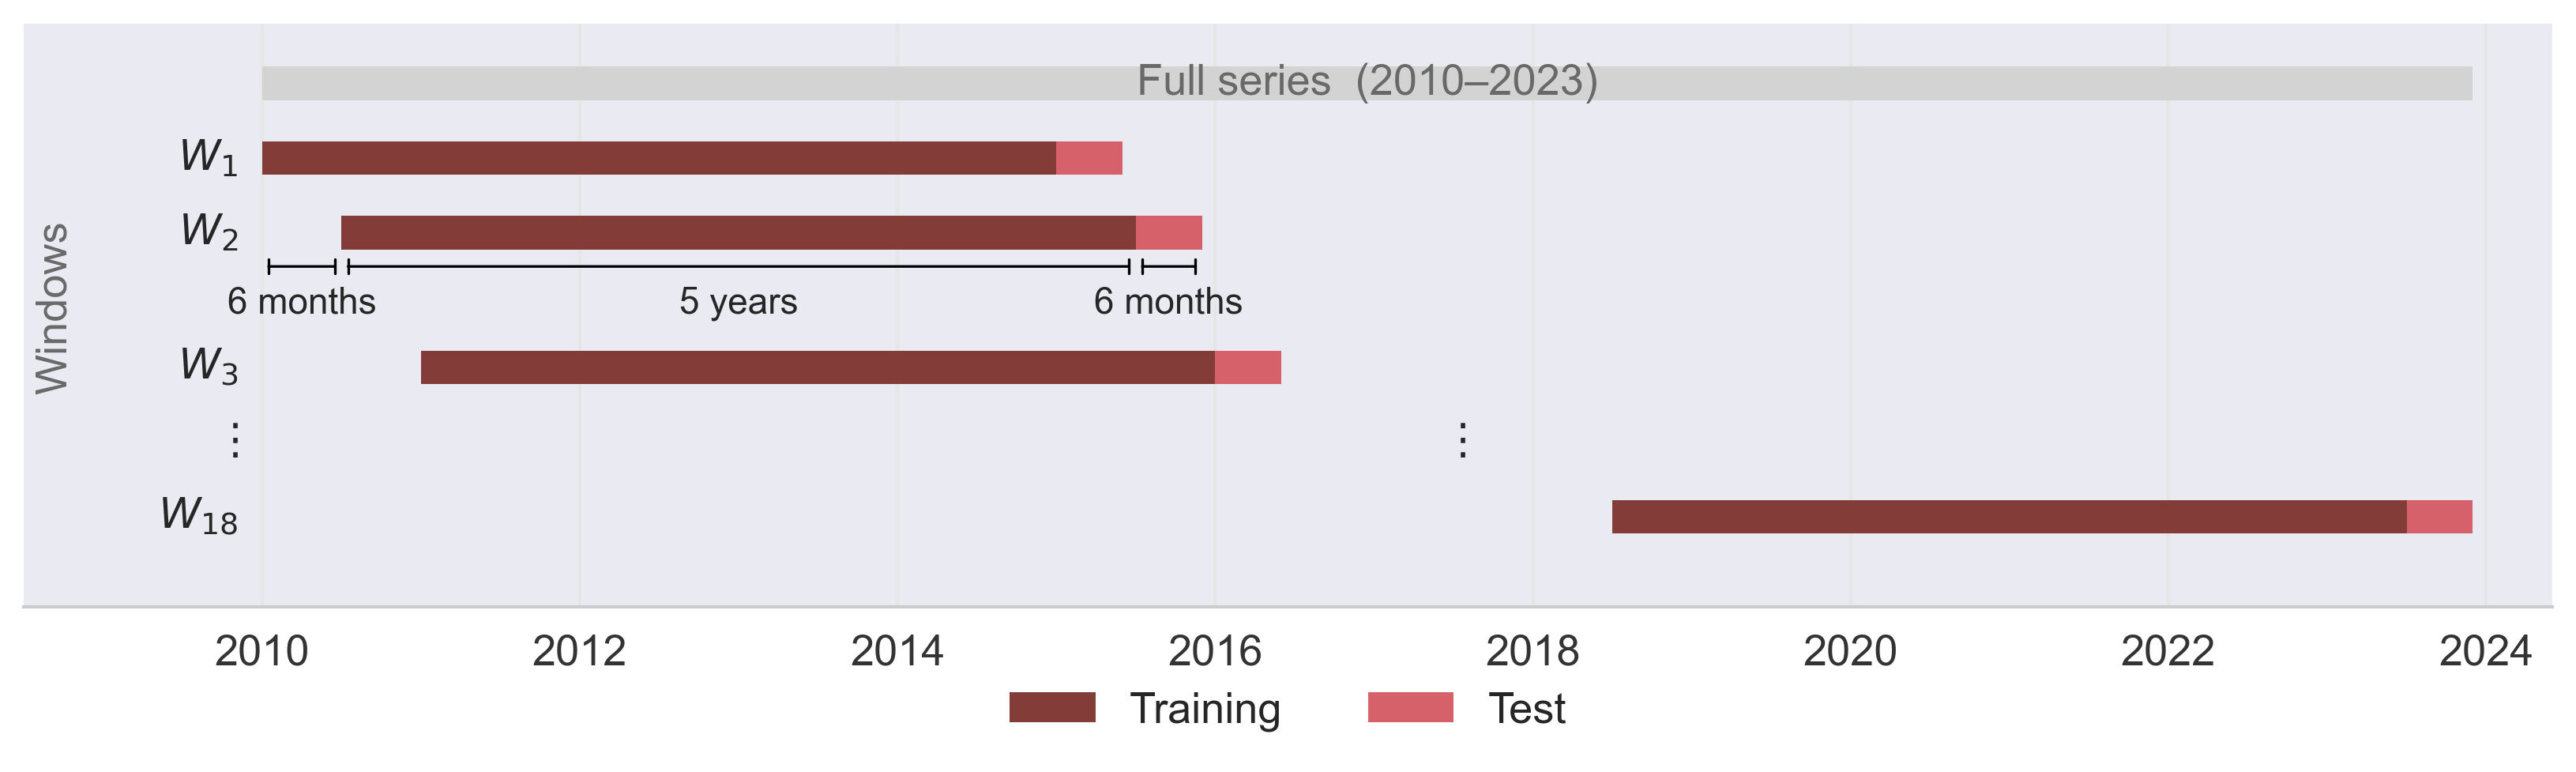
\includegraphics[width=\textwidth]{Figures/thesis_results/ExtraFigures/rolling_window_diagram.png}
    \caption{Rolling window evaluation design over the full sample period (2010--2024). Each window consists of a five-year training period followed by a six-month test period, with the window sliding forward by six months at a time, yielding 18 non-overlapping out-of-sample test periods.}
    \label{fig:rolling_window_diagram}

\end{figure}

For each rolling window, the in-sample RMSE is computed on the five-year training period and the out-of-sample RMSE on the subsequent six-month test period, providing a measure of how well the model generalises beyond the training sample. Figure~\ref{fig:Q2b} compares this generalisation gap across all models.
\begin{figure}[h]
    \centering
    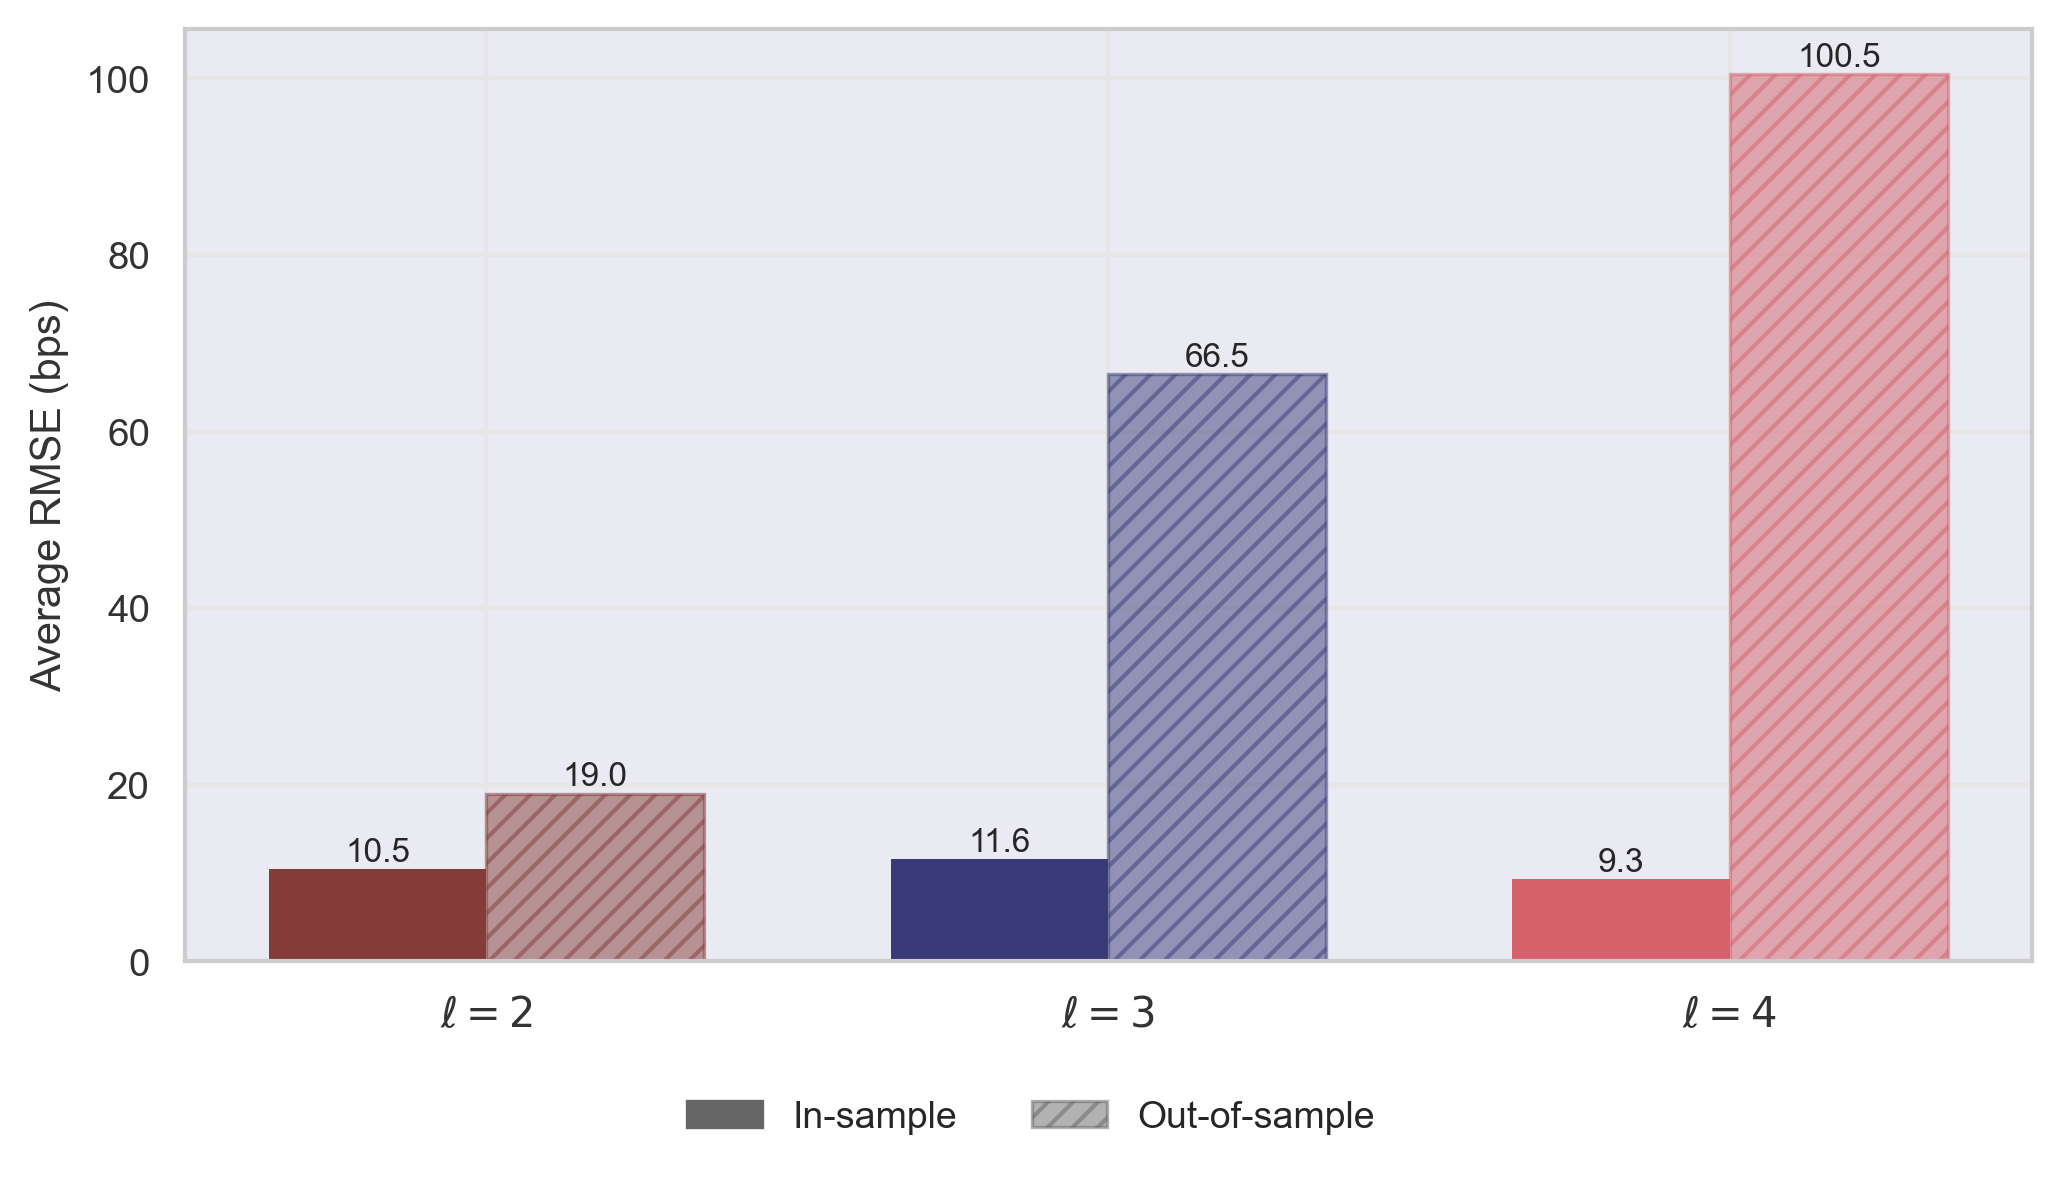
\includegraphics[width=.80\textwidth]{Figures/thesis_results/AutoencoderPerformance/Q2b_rolling_oos_vs_dim.png}
    %\caption{In-sample and rolling out-of-sample RMSE (bps) for models with $\ell \in \{2, 3, 4\}$ latent factors, averaged across all 18 rolling windows.}
    \caption{In-sample and rolling out-of-sample RMSE (bps) for models with $\ell \in \{2, 3, 4\}$ latent factors, averaged across all 18 rolling windows.  In-sample errors are similar across models, but the out-of-sample gap widens with latent dimension, indicating overfitting for \(\ell=3\) and \(\ell=4\).}
    \label{fig:Q2b}
\end{figure}

For latent dimensions greater than two, a substantial gap between in-sample and out-of-sample reconstruction accuracy is observed, indicative of overfitting. All models achieve average in-sample RMSEs between 9.3 and 11.6 bps, yet out-of-sample performance worsens markedly with the number of latent factors. The $\ell=2$ model increases from 10.5 bps to 19.0 bps out-of-sample, while the $\ell=3$ and $\ell=4$ models perform considerably worse out-of-sample, reaching 66.5 and 100.5 bps, respectively. Additional latent factors thus reduce in-sample error at the cost of out-of-sample generalisation. It is worth noting that the in-sample RMSEs are, on average, of similar magnitude to those reported in Section \ref{sec:ISevaluation}, suggesting that the models achieve reasonable reconstruction accuracy even when trained on shorter five-year windows with less data.

%\begin{table}[H]
%\centering
%{\small
%\pgfplotstableread[col sep=comma]{Figures/thesis_results/AutoencoderPerformance/Q4a_AE_vs_Kalman_OOS.csv}\datqfoura
%\resizebox{\textwidth}{!}{%
%\pgfplotstabletypeset[
%  columns={Model, Set, AUD, CAD, DKK, EUR, JPY, NOK, SEK, GBP, USD, Average, Time (min)},
%  columns/Model/.style={column name={Model}, string type, column type=l},
%  columns/Set/.style={column name={Set}, string type, column type=l},
%  columns/AUD/.style={column type=r, fixed, precision=2, fixed zerofill},
%  columns/CAD/.style={column type=r, fixed, precision=2, fixed zerofill},
%  columns/DKK/.style={column type=r, fixed, precision=2, fixed zerofill},
%  columns/EUR/.style={column type=r, fixed, precision=2, fixed zerofill},
%  columns/JPY/.style={column type=r, fixed, precision=2, fixed zerofill},
%  columns/NOK/.style={column type=r, fixed, precision=2, fixed zerofill},
%  columns/SEK/.style={column type=r, fixed, precision=2, fixed zerofill},
%  columns/GBP/.style={column type=r, fixed, precision=2, fixed zerofill},
%  columns/USD/.style={column type=r, fixed, precision=2, fixed zerofill},
%  columns/Average/.style={column name={\textbf{Avg.}}, column type=r, fixed, precision=2, fixed zerofill},
%  columns/Time (min)/.style={column name={\textbf{Time (min)}}, column type=r, fixed, precision=2, fixed zerofill},
%  every head row/.style={before row=\toprule, after row=\midrule},
%  every row no 2/.style={before row=\midrule},
%%  every row no 4/.style={before row=\midrule},
%  every last row/.style={after row=\bottomrule},
%]{\datqfoura}}
%}
%\caption{Rolling out-of-sample RMSE (bps) per currency for the autoencoder grouped by
%number of latent factors $\ell \in \{2, 3, 4\}$. For each $\ell$, IS shows the average
%in-sample RMSE across rolling windows and OOS shows the average rolling out-of-sample
%RMSE. The final column reports average training time per rolling window in minutes, reported on %the OOS row for each specification.}
%\label{tab:Q4a}
%\end{table}



To examine whether the out-of-sample errors are concentrated in particular periods, Figure~\ref{fig:Q3b} plots the rolling out-of-sample RMSE over time alongside the share of negative and inverted curves in both the training and test sets. The largest spikes coincide with periods where the test set contains a higher share of negative or inverted curves relative to the training set, most notably around 2016 and the rate-hiking cycle beginning in 2022. This suggests that what drives out-of-sample errors is not the amount of training data, but rather whether the curve types encountered at test time are well represented in the training window. 

\begin{figure}[H]
    \centering
    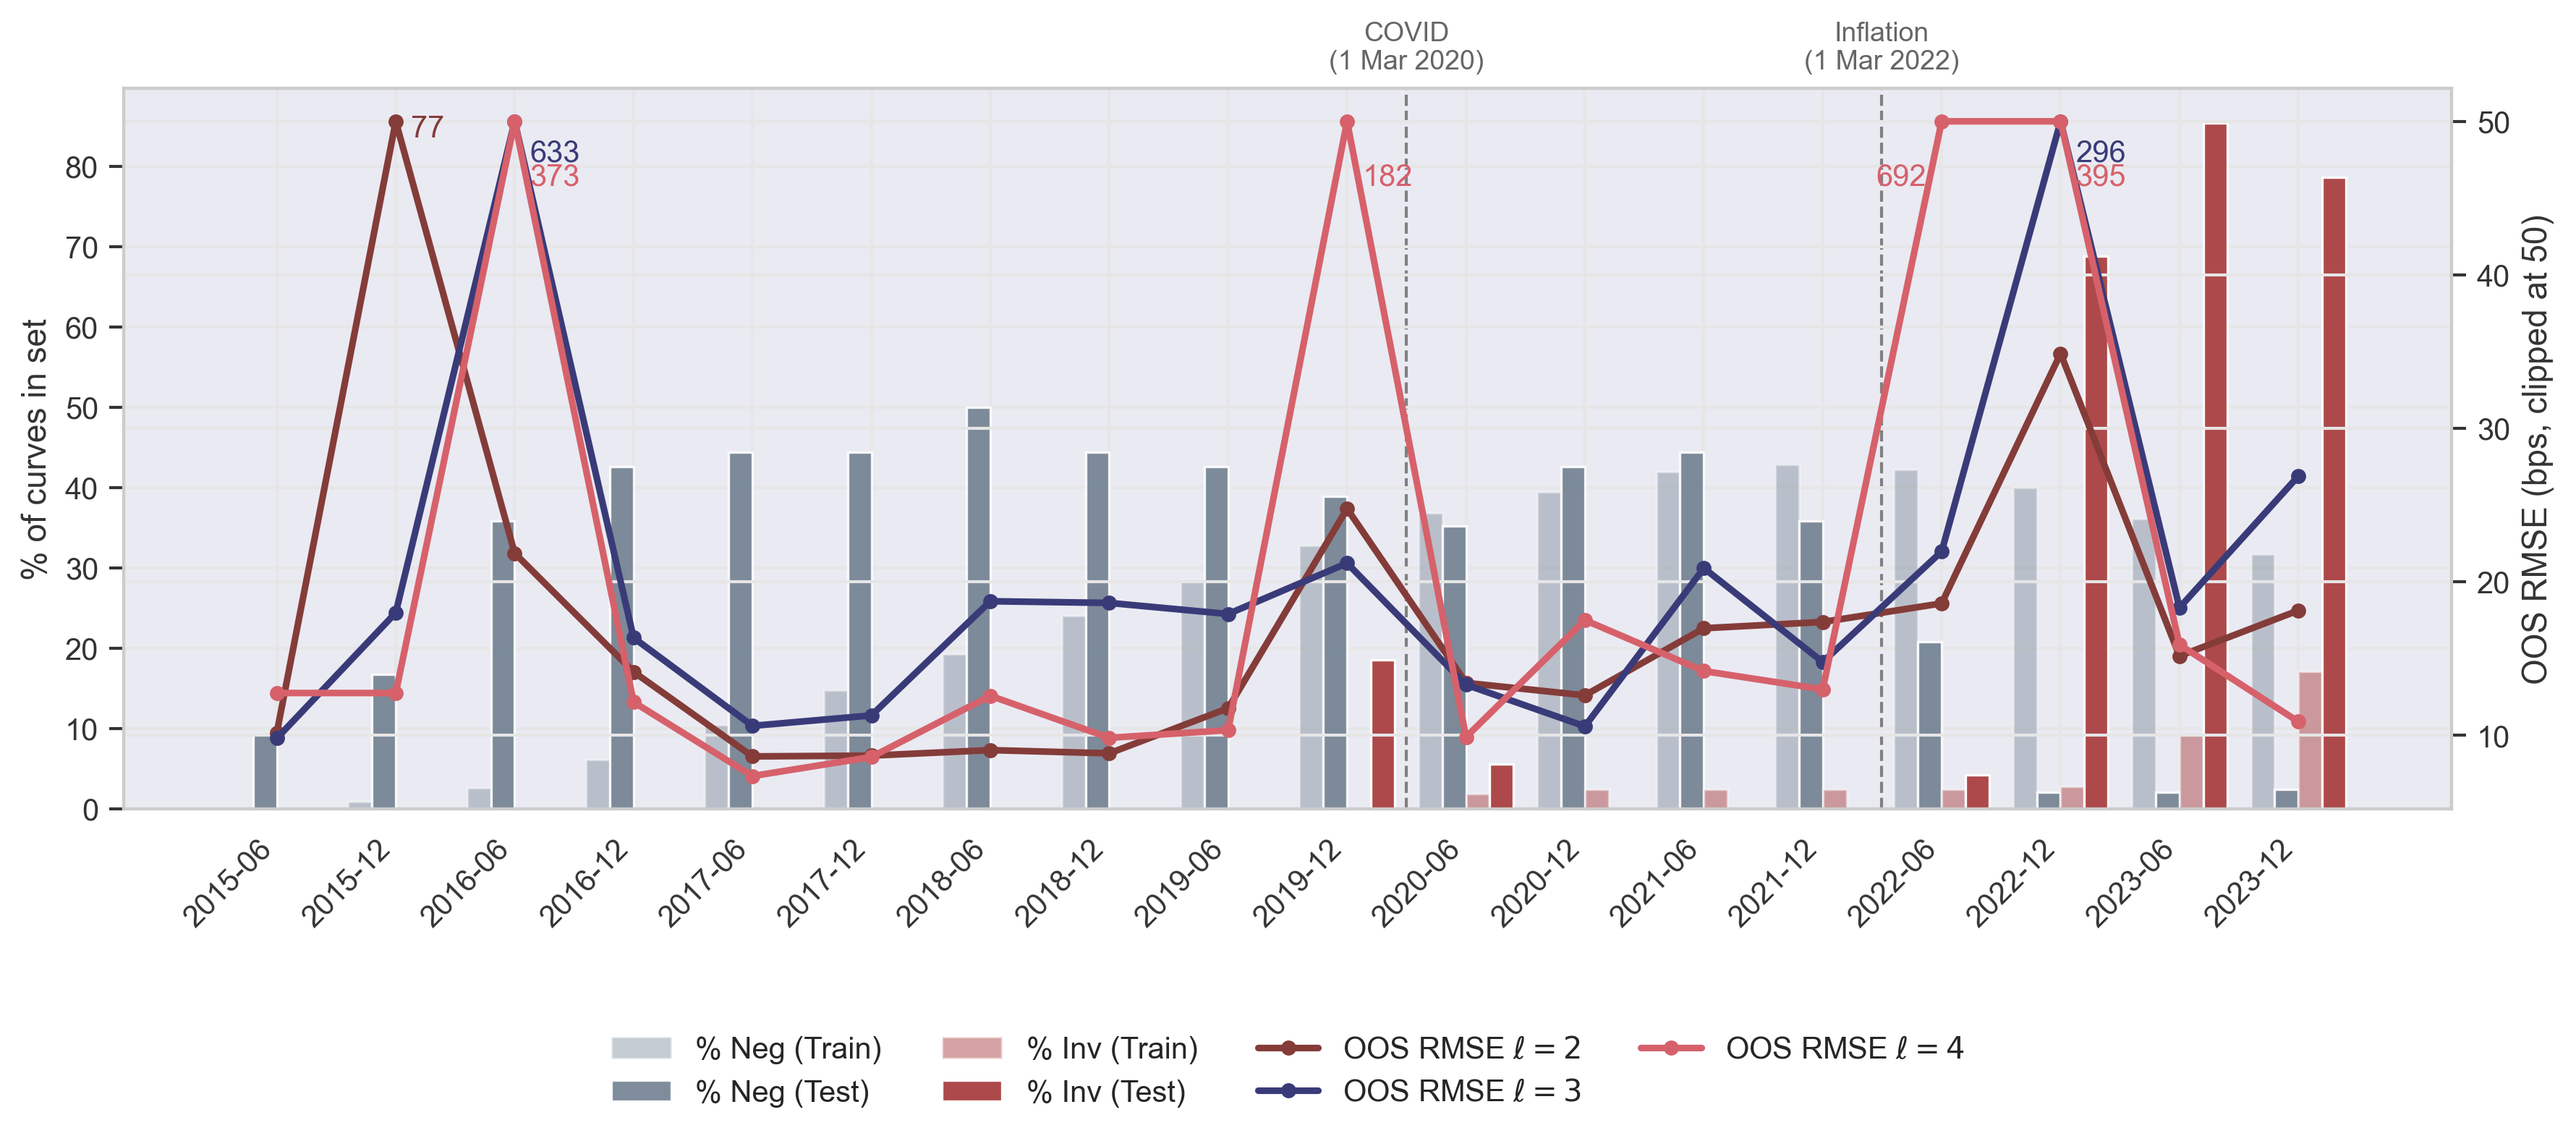
\includegraphics[width=1.02\textwidth]{Figures/thesis_results/AutoencoderPerformance/Q8a_rolling_regime_dual_axis.png}
    %\caption{Rolling out-of-sample RMSE (bps, right axis) for models with $\ell \in \{2, 3, 4\}$ latent factors, clipped at 50\,bps; true values are annotated where clipping occurs. Bars (left axis) show the percentage of negative-rate and inverted curve types in the training and test set of each rolling window. Dashed vertical lines mark the onset of macroeconomic regimes.}
    \caption{Rolling out-of-sample RMSE (bps, right axis) for models with $\ell \in \{2, 3, 4\}$ latent factors, clipped at 50\,bps; true values are annotated where clipping occurs. Bars (left axis) show the percentage of negative-rate and inverted curve types in the training and test set of each
    rolling window. Dashed vertical lines mark the onset of macroeconomic regimes. OOS errors spike when the test set contains a higher share of these curve types than the training window, with higher-dimensional models being most sensitive.}
    \label{fig:Q3b}
\end{figure}
% changed this figure from Q3b to Q8a

The higher-dimensional models are particularly sensitive to curve shapes underrepresented in the training data, as illustrated by the December 2019 window where inverted curves appear in the test set despite being absent from the training window, causing the $\ell=4$ model to spike to 182 bps while $\ell=2$ is considerably less affected. The sensitivity becomes even more apparent during the worst windows in the sample. Around 2016, when negative-rate curves begin appearing in the test sets after being largely absent from training, the $\ell=4$ model reaches 373 bps. Around 2022, where inverted curves surge in the test sets, the same model records errors of 692 and 395 across multiple windows. Across both periods, the high-dimensional models exhibit ont only larger peak errors but also more frequent spikes than their lower-dimensional counterparts.


To assess this more directly, Table~\ref{tab:q4c_oos_combined} breaks down the generalisation gap by curve type for the $\ell=2$ model across all rolling windows. The gap is modest for normal curves, with RMSE increasing from 8.4 to 11.4~bps. It is larger for inverted curves, from 14.9 to 20.4~bps and largest for negative-rate curves, where RMSE nearly doubles from 12.9 to 23.5~bps, supporting the claim that the model systematically struggles with curve types that are scarce in the training data.


\begin{table}[H]
\centering
{\small
\pgfplotstableread[col sep=comma]{Figures/thesis_results/AutoencoderPerformance/Q4c_oos_rmse_combined_display_transposed.csv}\datqfourcT
\pgfplotstabletypeset[
  columns={Metric, Normal, Inverted, Negative, Average},
  columns/Metric/.style={column name={}, string type, column type=l},
  columns/Normal/.style={string type, column type=r},
  columns/Inverted/.style={string type, column type=r},
  columns/Negative/.style={string type, column type=r},
  columns/Average/.style={column name={\textbf{Average}}, string type, column type=r},
  every head row/.style={before row=\toprule, after row=\midrule},
  every last row/.style={after row=\bottomrule},
]{\datqfourcT}
}
%\caption{In-sample and out-of-sample RMSE (bps) by curve type for the model with $\ell = 2$ latent factors, aggregated across all currencies. IS RMSE is averaged over the training sets and OOS RMSE over the test sets across all 18 rolling windows. Curve type definitions follow Table~\ref{tab:curve_type_counts}.}
\caption{In-sample and out-of-sample RMSE (bps) by curve type for the model with $\ell = 2$ latent factors, aggregated across all currencies. IS RMSE is averaged over the training sets and OOS RMSE over the test sets across all 18 rolling windows. The generalisation gap is modest for normal curves but grows substantially for inverted and negative-rate curves, reflecting limited training exposure to these curve shapes.}
\label{tab:q4c_oos_combined}
\end{table}


To summarise, models with more than two latent dimensions overfit out-of-sample, and underrepresented curve types yield larger errors. 






